\documentclass{article}
\usepackage{amsmath,amssymb,amsthm,graphicx,xcolor,url,hyperref,mathrsfs,enumitem,thmtools}
\usepackage[numbers,sort&compress]{natbib}
\newtheorem{theorem}{Theorem}\newtheorem{lemma}[theorem]{Lemma}\newtheorem{proposition}[theorem]{Proposition}\newtheorem{corollary}[theorem]{Corollary}\newtheorem{definition}[theorem]{Definition}\newtheorem{claim}[theorem]{Claim}\newtheorem{remark}[theorem]{Remark}\newtheorem{example}[theorem]{Example}\newtheorem*{claim*}{Claim}
\author{Emmanuel Filiot \and Ismaël Jecker \and Christof Löding \and Anca Muscholl \and Gabriele Puppis \and Sarah Winter}\date{}



%\usepackage{amsmath}
%\usepackage{amssymb}
%\usepackage{fullpage}
%\usepackage{amsthm}
%\usepackage{thmtools}
\usepackage{thm-restate} % allows repeating theorems, lemmas, etc.
%\usepackage{suffix} % enables definitions of macros with *
\usepackage{tikz}
%\usepackage{subcaption} % subfigures with their own caption
%\usepackage{enumitem} % custom enumerate environments
%\setlength{\marginparwidth}{2cm}
%\usepackage[textwidth=15mm,textsize=scriptsize]{todonotes}
%\usepackage{orcidlink}
\providecommand{\AP}{}\NewDocumentCommand{\reintro}{o m}{#2}
\usepackage{xspace}
\usepackage{mathrsfs}


%% comments
% \newrobustcmd{\anca}[2][]{{\color{black}\todo[color=cyan!30,noshadow,#1]{{\bf Anca:} #2}}\ignorespaces}
% \newrobustcmd{\manu}[2][]{{\color{black}\todo[color=blue!30,noshadow,#1]{{\bf Manu:} #2}}\ignorespaces}
% \newrobustcmd{\gabriele}[2][]{{\color{black}\todo[color=magenta!25,noshadow,#1]{{\bf Gabriele:} #2}}\ignorespaces}
% \newrobustcmd{\ismael}[2][]{{\color{black}\todo[color=green!20,noshadow,#1]{{\bf Ismael:} #2}}\ignorespaces}
% \newrobustcmd{\isma}[2][]{{\color{black}\todo[color=green!20,noshadow,#1]{{\bf Ismael:} #2}}\ignorespaces}
% \newrobustcmd{\sarah}[2][]{{\color{black}\todo[color=yellow!20,noshadow,#1]{{\bf Sarah:} #2}}\ignorespaces}
% \newrobustcmd{\christof}[2][]{{\color{black}\todo[color=orange!30,noshadow,#1]{{\bf Christof:} #2}}\ignorespaces}


% knowledge setup
\definecolor{ThCSdarkblue}{RGB}{25,34,64}
% notion styling adapted to plain text
% notion styling adapted to plain text
%\knowledgestyle*{notion}{underline}
%\knowledgestyle*{unknown}{color=nicered}


%%TheoretiCS Restating Theorems%%%%%
\newcommand{\RestateRemark}[1]{{\normalfont\bfseries #1}}
\newcommand{\RestateInit}[1]{\newcommand{#1}{}}
\newcommand{\RestateGo}[1]{\renewcommand{#1}{(Restated)}}


% environments
% \newtheorem{claim}{Claim}
% \newtheorem*{claim*}{Claim}
% \newtheorem{remark}{Remark}
% \newtheorem{example}{Example}
% \newtheorem{definition}{Definition}
% \newtheorem{theorem}{Theorem}
% \newtheorem{proposition}[theorem]{Proposition}
% \newtheorem{corollary}[theorem]{Corollary}
% \newtheorem{lemma}[theorem]{Lemma}


% nicer colors
\definecolor{darkblue}{RGB}{0,0,92}
\definecolor{nicecyan}{HTML}{006165}
\definecolor{nicered}{HTML}{DB3A34}
\definecolor{nicegreen}{HTML}{6D972E}
\newcommand\nicecyan[1]{{\color{nicecyan}#1}}
\newcommand\nicered[1]{{\color{nicered}#1}}
\newcommand\nicegreen[1]{{\color{nicegreen}#1}}


% tikz
\usetikzlibrary{calc}
\usetikzlibrary{patterns}
\usetikzlibrary{decorations}
\usetikzlibrary{decorations.markings}
\usetikzlibrary{decorations.pathmorphing}
\usetikzlibrary{decorations.pathreplacing}
\usetikzlibrary{backgrounds}
\usetikzlibrary{arrows}
\usetikzlibrary{arrows.meta}
\usetikzlibrary{bending}

\tikzset{every node/.style={font=\vphantom{Ag}, minimum size=1mm, inner sep=0pt, outer sep=0pt}}
\tikzset{every path/.style={line width=0.5pt, shorten >=3pt, shorten <=3pt}} % if modified, it remember to modify it also below

\tikzstyle{dot}=[draw, shape=circle, fill, style={font=\vphantom{}}]
\tikzstyle{bluebox}=[shape=rectangle, fill=cyan!50, minimum size=4mm, inner sep=2pt, outer sep=0pt]
\tikzstyle{ubrace} = [draw, thick, decoration={brace, mirror, raise=0.0cm}, decorate, 
                      every node/.style={anchor=north, yshift=-0.1cm}]

\tikzstyle{outline} = [preaction={-, draw, shorten >=2pt, shorten <=2pt, line width=2pt, white}]

\tikzstyle{arrow} = [arrows = {->[bend,round,scale=1.5]}]
\tikzstyle{directededge} = [arrows = {-latex'}]
\tikzstyle{over} = [preaction={-, draw, shorten >=1pt, shorten <=1pt, line width=5pt, white}]
\tikzstyle{partialarrow} = [arrows = {->[bend,round,scale=1.5,harpoon]}]
\tikzstyle{surjectivearrow} = [arrows = {-To[bend,round,scale=1.5]To[bend,round,scale=1.5]}]
\tikzstyle{injectivearrow} = [arrows = {>[bend,round,scale=1.5]->[bend,round,scale=1.5]}]
\tikzstyle{mapsto} = [|->]

\tikzstyle{loop above} = [loop, looseness=15, out=50, in=130]
\tikzstyle{loop below} = [loop, looseness=15, out=230, in=310]
\tikzstyle{loop left} = [loop, looseness=15, out=140, in=220]
\tikzstyle{loop right} = [loop, looseness=15, out=-40, in=40]

\NewDocumentCommand{\mygrid}{}{
	\begin{pgfonlayer}{background}
		\draw [help lines, red!5, step=0.25] (current bounding box.south west) grid (current bounding box.north east);
		\draw [help lines, red!25, step=1] (current bounding box.south west) grid (current bounding box.north east);
		\node [help lines, red, dot] (0,0) {};
	\end{pgfonlayer}
}

\NewDocumentCommand{\myclip}{s m m}{
	\tikzset{every path/.style={}}
	\clip (#2) rectangle (#3);
	\IfBooleanTF{#1}{
		\draw [help lines, red] (#2) rectangle (#3);
		\mygrid
	}{}
	\tikzset{every path/.style={line width=0.5pt, shorten >=3pt, shorten <=3pt}}
}



\newcommand{\unif}[1]{\textsf{Unif}(#1)}
\newcommand{\refine}[1]{\textsf{Refine}(#1)}
\newcommand{\outp}[1]{\out{#1}}
\newcommand{\aut}{A}
\newcommand{\sst}{T}



\renewcommand{\a}{\alpha}
\renewcommand{\b}{\beta}
\newcommand{\g}{\gamma}
\newcommand{\e}{\eta}
\newcommand{\w}{\omega}
\newcommand{\act}[1]{\stackrel{#1}{\longrightarrow}}

\newcommand{\var}{\mathcal{X}}
\newcommand{\varO}{O}
\newcommand{\alp}{\Sigma}
\newcommand{\idsub}[1]{\textsf{Id}_{#1}}
\newcommand{\sub}[2]{{\mathcal S}_{#1,#2}}

\NewDocumentCommand{\out}{s m}{\IfBooleanTF{#1}{
	 \operatorname{out}(#2)}{
	\operatorname{out}(#2)}}

\newcommand{\finalupd}{O}




\newcommand{\run}[2]{\wrun[#1]{#2}}
\newcommand{\runA}[2]{\lrun[#1]{#2}}
\newcommand{\runB}[2]{\mrun[#1]{#2}}
\newcommand{\runC}[2]{\rrun[#1]{#2}}



\let\oldotimes\otimes
\RenewDocumentCommand{\otimes}{s}{\IfBooleanTF{#1}{
	 \mathbin{\oldotimes}}{
	 \mathbin{\oldotimes}}}

\NewDocumentCommand{\inp}{s m}{\IfBooleanTF{#1}{
	 \operatorname{in}(#2)}{
	 \operatorname{in}(#2)}}

\NewDocumentCommand{\rel}{s m}{\IfBooleanTF{#1}{
	 \mathscr{R}(#2)}{
	 \mathscr{R}(#2)}}


\NewDocumentCommand{\rt}{s m}{\IfBooleanTF{#1}{
	 \operatorname{root}(#2)}{
	\operatorname{root}(#2)}}


\NewDocumentCommand{\Cover}{s O{C,D} m}{\IfBooleanTF{#1}{
	 \operatorname{Cover}_{#2}(#3)}{
	\operatorname{Cover}_{#2}(#3)}}


\NewDocumentCommand{\lrun}{s O{P} m}{\IfBooleanTF{#1}{
	 \operatorname{lft}\nolimits_{#2}^{#3}}{
	\operatorname{lft}\nolimits_{#2}^{#3}}}

\NewDocumentCommand{\mrun}{s O{P} m}{\IfBooleanTF{#1}{
	 \operatorname{mid}\nolimits_{#2}^{#3}}{
	\operatorname{mid}\nolimits_{#2}^{#3}}}

\NewDocumentCommand{\rrun}{s O{P} m}{\IfBooleanTF{#1}{
	 \operatorname{rgt}\nolimits_{#2}^{#3}}{
	\operatorname{rgt}\nolimits_{#2}^{#3}}}

\NewDocumentCommand{\wrun}{s O{P} m}{\IfBooleanTF{#1}{
	 \operatorname{run}\nolimits_{#2}({#3})}{
	\operatorname{run}\nolimits_{#2}({#3})}}


\NewDocumentCommand{\seqprj}{s m}{\IfBooleanTF{#1}{
	 #2^\star}{
	#2^\star}}


\NewDocumentCommand{\pairprj}{s m}{\IfBooleanTF{#1}{
	 #2^\star}{
	#2^\star}}






\NewDocumentCommand{\flow}{s m}{\IfBooleanTF{#1}{
	 \operatorname{flow}(#2)}{
	\operatorname{flow}(#2)}}

\NewDocumentCommand{\pump}{s D<>{2} O{L} m}{\IfBooleanTF{#1}{
	 \operatorname{pump}^{#2}_{#3}(#4)}{
  	\operatorname{pump}^{#2}_{#3}(#4)}}



\NewDocumentCommand{\formal}{m}{\mathtt{#1}}

\NewDocumentCommand{\sol}{s m}{\IfBooleanTF{#1}{
	 \operatorname{Sols}(#2)}{
	\operatorname{Sols}(#2)}}

\NewDocumentCommand{\plex}{s m}{\IfBooleanTF{#1}{
	 \le_{#2}}{
	\mathrel{\le_{#2}}}}
	
\NewDocumentCommand{\pgex}{s m}{\IfBooleanTF{#1}{
	 \ge_{#2}}{
	\mathrel{\ge_{#2}}}}
	
\NewDocumentCommand{\pleY}{s m}{\IfBooleanTF{#1}{
	 \le_{#2}}{
	\mathrel{\le_{#2}}}}
	
\NewDocumentCommand{\pgeY}{s m}{\IfBooleanTF{#1}{
	 \ge_{#2}}{
	\mathrel{\ge_{#2}}}}
	
\NewDocumentCommand{\ple}{s}{\IfBooleanTF{#1}{
	 \le}{
	\mathrel{\le}}}
	
\NewDocumentCommand{\pge}{s}{\IfBooleanTF{#1}{
	 \ge}{
	\mathrel{\ge}}}

\NewDocumentCommand{\pdot}{s}{\IfBooleanTF{#1}{
	 \cdot}{
	\mathbin{\cdot}}}

\NewDocumentCommand{\pdotY}{s m}{\IfBooleanTF{#1}{
	 \cdot_{#2}}{
	\mathbin{\cdot_{#2}}}}




\NewDocumentCommand{\weight}{s O{u} O{v} m}{\IfBooleanTF{#1}{
	 \operatorname{weight}^{#2}_{#3}(#4)}{
  	\operatorname{weight}^{#2}_{#3}(#4)}}

%\NewDocumentCommand{\diff}{s O{\rho,\rho'} m}{\IfBooleanTF{#1}{
%	 \operatorname{diff}_{#2}(#3)}{
%  	\operatorname{diff}_{#2}(#3)}}

%\NewDocumentCommand{\lag}{s O{\rho,\rho'} m}{\IfBooleanTF{#1}{
%	 \operatorname{lag}_{#2}(#3)}{
%  	\operatorname{lag}_{#2}(#3)}}

\NewDocumentCommand{\period}{s m}{\IfBooleanTF{#1}{
	 \operatorname{period}(#2)}{
  	\operatorname{period}(#2)}}

\NewDocumentCommand{\cuts}{s D<>{C} m}{\IfBooleanTF{#1}{
	 {#2}\mspace{-3mu}\operatorname{-cuts}(#3)}{
  	{#2}\mspace{-3mu}\operatorname{-cuts}(#3)}}

\NewDocumentCommand{\delay}{s D<>{C} m}{\IfBooleanTF{#1}{
	 {#2}\mspace{-3mu}\operatorname{-delay}(#3)}{
  	{#2}\mspace{-3mu}\operatorname{-delay}(#3)}}
  	
  	
\let\oldiota\iota
\RenewDocumentCommand{\iota}{s}{\IfBooleanTF{#1}{
	 \oldiota}{
  	\oldiota}}



\NewDocumentCommand{\Sep}{s O{C,D} m}{\IfBooleanTF{#1}{
	 \operatorname{Sep}_{#2}(#3)}{
	\operatorname{Sep}_{#2}(#3)}}












    
	

    






	















%\knowledge{notion}
%	| projection
%	| projections


%
%\knowledge{notion}
% notion registry omitted
% notion registry omitted
% notion registry omitted















	










	

































\title{Finite-valued Streaming String Transducers}



          
% \author{
% \orcidlink{https://orcid.org/0000-0002-2520-5630}
%     Emmanuel Filiot (Université libre de Bruxelles, Belgium)\\
% \orcidlink{https://orcid.org/0000-0002-6527-4470}
%     Ismaël Jecker (Université de Besançon, France)\\
% \orcidlink{https://orcid.org/0000-0001-9831-3264} 
%     Gabriele Puppis (University of Udine, Italy)\\
% \orcidlink{https://orcid.org/0000-0002-1529-2806}
%     Christof Löding (RWTH Aachen University, Germany)\\
% \orcidlink{https://orcid.org/0000-0002-8214-204X}
%     Anca Muscholl (LaBRI, Université Bordeaux, France)\\
% \orcidlink{https://orcid.org/0000-0002-3499-1995}
%     Sarah Winter (IRIF, Université Paris Cité, France)
% }
% \date{}



%%%%%%%%%%%%%%%%%%%%%%%%%%%%%%%%%%%%%%%%%%%%%%%%%%%%%%
%% EDITORIAL
%%%%%%%%%%%%%%%%%%%%%%%%%%%%%%%%%%%%%%%%%%%%%%%%%%%%%%



%\ThCSrevised{??} %there was no revision request





\begin{document}

\maketitle


\begin{abstract}
       A  transducer is finite-valued if there exists a bound
    $k$ such that any given
    input maps to at most $k$ outputs. For classical
    one-way transducers, it is known since the 1980s that
    finite valuedness entails decidability of the equivalence
    problem. This result is in contrast with undecidability in the
    general case, making finite-valued transducers
    very appealing. For one-way transducers it is also known that
    finite valuedness itself is decidable and that any
    $k$-valued finite transducer can be decomposed into a union of $k$
    single-valued finite transducers. 


    In this article, we extend the above results to copyless streaming string
    transducers (SSTs), addressing open questions raised by Alur and
    Deshmukh in 2011. SSTs strictly extend the expressiveness of
    one-way transducers via additional variables that store
    partial outputs. We prove that any $k$-valued SST can be
    effectively decomposed into a union of $k$ (single-valued)
    deterministic SSTs. As a corollary, we establish the equivalence
    between SSTs and two-way transducers in the finite-valued case, even though these models are generally incomparable. Another corollary provides an elementary upper bound for
    deciding equivalence of finite-valued SSTs. The equivalence problem was already
    known to be decidable, but the proof complexity relied
    on Ehrenfeucht's
    conjecture. Lastly, our main contribution shows that finite valuedness of SSTs is
    decidable, with the complexity  being {\upshape\sc PSpace} in general, and  {\upshape\sc PTime} when the
    number of variables is fixed.  
\end{abstract}

 


\section{Introduction}\label{sec:intro}
\enlargethispage{-\baselineskip}
Finite-state word transducers are simple devices that allow 
effective reasoning about data transformations. 
In their most basic form, they transform words using finite control. 
\AP
For example, the oldest transducer model, 
known as generalized sequential machine, 
extends deterministic finite state automata by associating each input with a corresponding output
that is generated by appending finite words specified along the transitions.
This rather simple model of transducer is capable of representing 
basic partial functions between words, e.g.~the left 
rotating function $a_1\: a_2\dots a_n\mapsto a_2\dots a_n \: a_1$.
\AP
Like automata, transducers can also be enhanced with non-determinism,
as well as the ability of scanning the input several times (two-wayness).
\AP
For example, the non-deterministic counterpart of 
generalized sequential machines, called here one-way transducers, 
can be used to represent the right rotating function 
$a_1\dots a_{n-1}\: a_n\mapsto a_n\:a_1\dots a_{n-1}$,
but also word relations that are not partial functions, like for 
instance the relation that associates an input $a_1\dots a_n$ 
with any output from $\{a_1\}^*\dots \{a_n\}^*$.
Similarly, deterministic two-way transducers can compute 
the mirror function $a_1\dots a_n \mapsto a_n\dots a_1$,
the squaring function $w \mapsto w w$, etc.

\AP
Inspired by a logic-based approach applicable to arbitrary relational structures~\cite{CE12}, 
MSO-definable word transductions were considered by Engelfriet and
Hoogeboom~\cite{eh01} and shown to be equivalent to deterministic 
two-way transducers.
\AP
Ten years later Alur and Cern{\'y}~\cite{DBLP:conf/fsttcs/AlurC10} proposed 
\reintro{streaming string transducers} (\reintro{SSTs} for short), 
a one-way model that uses write-only variables as additional storage. 
In SSTs, variables store strings and  can be updated by appending or prepending strings, or 
concatenated together, but not duplicated (they are copyless). 
Alur and Cern{\'y} also showed that, in the functional case, 
that is, when restricting to transducers that represent partial functions,
SSTs are equivalent to the model studied in~\cite{eh01},
and thus in particular to two-way transducers.
These equivalences between transducer models motivate nowadays 
the use of the term ``regular'' word function, in the spirit of
classical results on regular word languages from automata theory 
and logics due to B\"uchi, Elgot, Trakhtenbrot, Rabin, and others. 

While transducers inherit features like
non-determinism and two-wayness from automata,
these characteristics have an
impact on their expressive power compared to automata. 
In the case of automata it is known that adding non-determinism and 
two-wayness does not affect the expressive power,
as it only makes them more succinct in terms of number of states.
It does not affect decidability of fundamental problems either,
though succinctness makes some problems 
computationally harder. 
In contrast, for transducers, non-determinism 
and/or two-wayness
significantly  change the expressive power.
For instance, non-deterministic one-way transducers may capture 
relations that are not partial functions,
and thus not computable by generalized sequential machines\footnote{Even if a
non-deterministic one-way transducer computes a partial function, there may be
no equivalent deterministic one-way transducer. However, this question can be decided in {\upshape\sc PTime}~\cite{BealC02,AllauzenM03}.}.
This difference is also apparent at the level of decidability results. 
For example, the equivalence problem is in {\upshape\sc NLogSpace}
for generalized sequential machines,
and undecidable for one-way transducers \cite{FischerR68,iba78siam,many_facets}.
We should also mention that in the functional case it is 
possible to convert one transducer model to another
(e.g.~convert an SST to an equivalent two-way transducer).
In the non-functional case, the picture is less satisfactory.
In particular, non-deterministic SSTs and non-deterministic 
two-way transducers turn out to be incomparable:
for example, the relation
$\{(u\,v, \, v\,u) \::\: u,v\in\Sigma^*\}$ can be represented 
in the former model but not in the latter, while the relation
$\{(w, \, w^n) \::\: w\in\Sigma^*, n\in\mathbb{N}\}$ can be
represented in the latter model but not in the former.
\AP
However, SSTs can still be converted to equivalent
non-deterministic MSO transductions~\cite{DBLP:conf/icalp/AlurD11}, 
which extend the original MSO transductions 
by existentially quantified monadic parameters.


\AP
There is however a class of relations that is close
to (regular) word functions in terms of good behavior: 
the class of \reintro{finite-valued} relations.
These are relations that associate a uniformly bounded
number of outputs with each input.
%Of course, this class contains all the (regular) functions.
\AP
The concept of bounding the number of outputs associated 
with each input in a transducer is closely related to 
the notion of  \reintro{finite ambiguity}, which refers to bounding the number of accepting runs.
 Ambiguity has been intensively studied 
in the context of formal languages, where it is shown,
for instance, that equivalence of unambiguous
automata is decidable in {\upshape\sc PTime} \cite{Stearns1985OnTE}.
In the context of relations, $k$-valuedness and $k$-ambiguity
were initially considered in the setting of one-way transducers. 
For example, \cite{GI83} showed that, for fixed $k$,
one can decide in {\upshape\sc PTime} whether a given one-way transducer
is $k$-valued. Similarly, $k$-valuedness for fixed $k$ can be decided
in {\upshape\sc PSpace} for two-way transducers and SSTs~\cite{DBLP:conf/icalp/AlurD11}.


It is also clear that every $k$-ambiguous
one-way transducer is $k$-valued. 
Conversely, it was shown that every $k$-valued
one-way transducer can be converted to an 
equivalent, $k$-ambiguous one 
\cite{Weber93,web96,DBLP:journals/mst/SakarovitchS10}.
This result, even if it deals with a rather simple model
of transducer, already uses advanced normalization techniques 
from automata theory and involves an exponential
blow up in the number of states, as shown in the 
example below.

\begin{example}\label{ex:finitevalued}
    Fix $k\in\mathbb{N}$ and consider the relation
    \[
      R_k ~=~ 
      \big\{ 
        (w_1\dots w_n, \, w_i) \::\:
        n\in\mathbb{N}, \: 1\leq i\leq n, \:
        w_1,\dots,w_n \in \{0,1\}^k
      \big\}.
    \]
    Examples of pairs in this relation, for $k=2$, are 
    $(00\,10\,11,\,00)$, 
    $(00\,10\,11,\,10)$, and 
    $(00\,10\,11,\,11)$. 
    \AP
    For arbitrary $k$, the relation $R_k$ 
    associates at most $2^k$ outputs with each input
    (we say it is \reintro{$2^k$-valued}).
    This relation can be realized by one-way transducers
    that exploit non-determinism to guess which block from
    the input becomes the output. 
    For instance, a possible transducer $T_k$ that realizes $R_k$
    repeatedly consumes blocks of $k$ bits from the input, 
    without outputting anything, until it non-deterministically 
    decides to copy the next block, and after that it 
    continues consuming the remaining blocks without output.
    Note that this transducer $T_k$ has $\mathcal{O}(k)$
    states, it is finite-valued, but not finite-ambiguous,
    since the number of accepting runs per input 
    depends on the number $n$ of blocks in the input and it 
    is thus unbounded. 
    A finite-ambiguous transducer realizing the same relation
    $R_k$ can be obtained at the cost of an exponential blow-up
    in the number of states, 
    for instance by initially guessing and outputting a $k$-bit
    word $w$ (this requires at least $2^k$ states), 
    and then verifying that $w$ occurs 
    as a block of the input. 
\end{example}


Since $k$-ambiguous automata can be easily 
decomposed into a  union of $k$ unambiguous automata,
the possibility of converting a $k$-valued one-way transducer 
to a $k$-ambiguous one   entails a decomposition result of the 
following form: every $k$-valued one-way transducer is equivalent
to a finite union of functional one-way transducers.
One advantage of this type of decomposition is that it allows to generalize
the decidability of the equivalence problem from functional 
to $k$-valued one-way transducers,
which brings us back to the original motivation for considering 
classes of finite-valued relations.
Decidability of the equivalence problem for
$k$-valued one-way transducers was independently established
in~\cite{ck86}.
The latter work also states that the same techniques can be adapted 
to show decidability of equivalence for $k$-valued 
two-way transducers as well.
Inspired by~\cite{ck86}, the equivalence problem was later shown 
to be decidable also for $k$-valued SSTs~\cite{equivalence-finite-valued}.
However, the decidability results from~\cite{ck86} and~\cite{equivalence-finite-valued} 
rely on the Ehrenfeucht conjecture~\cite{AL85,Guba86} and therefore provide no elementary
upper bounds on the complexity. 



Decomposing finite-valued SSTs and deciding
finite valuedness for SSTs were listed as open problems 
in~\cite{DBLP:conf/icalp/AlurD11}, more than 10 years ago,
and represent our main contributions.
Compared to one-way transducers, new challenges arise with
SSTs, due to the extra power they enjoy to produce outputs. 
For example, consider the relation consisting of all pairs
of the form $(w, 0^{n_0}1^{n_1})$ or $(w, 1^{n_1}0^{n_0})$, 
where $w\in\{0,1\}^*$, and $n_b$ ($b=0,1$) is the number of 
occurrences of $b$ in $w$. 
%The outputs are essentially the
%concatenated numbers of $0$
%and $1$, in unary, and in any order. 
This relation is $2$-valued, and is not realizable by any one-way transducer. 
On the other hand, the relation is realized by an SST $T$ with a single state 
and two variables, denoted $X_0,X_1$ and both initially empty: 
whenever $T$ reads $b\in\{0,1\}$,
it non-deterministically applies the update $X_b := b \,X_b$ or 
$X_b := X_b\,b$ (while leaving $X_{1-b}$ unchanged); at the end of
the input, $T$ outputs either $X_0 \, X_1$ or $X_1 \, X_0$. 
The ability of SSTs to generate outputs in a non-linear way
makes their study challenging and intriguing. To illustrate this, 
consider a slight modification of $T$ where
$X_0$ is initialized with $1$, instead of the empty word:
the new SST is not finite-valued anymore, because upon 
reading $0^n$ it could output any word of the form 
$0^i \,1 \, 0^j$, with $i,j\in\mathbb{N}$ such that $i+j = n$. 



Another open problem was to compare the expressive power of SSTs and 
two-way transducers in the finite-valued case.
It is  not hard to see that the standard translation from deterministic
two-way transducers to deterministic SSTs also applies to the
finite-valued case (cf.~second part of the proof of Theorem~\ref{thm:finval-SST-2FT}).
The converse translation, however, is far more complicated and relies on
the decomposition theorem for SSTs which we establish in this article.



\medskip
\subparagraph*{\bf Contributions.} 
The results presented in this article  draw a
rather complete picture about 
finite-valued SSTs, answering several open problems from~\cite{DBLP:conf/icalp/AlurD11}.
First, we show that $k$-valued SSTs enjoy the same decomposition property as
one-way transducers:  
\RestateInit{\restateDecomposition}
\begin{restatable}{theorem}{Decomposition}
\label{thm:FiniteValuedToDecomposition}\RestateRemark{\restateDecomposition}
    For all $k \in \mathbb{N}$, 
    every $k$-valued SST can be effectively decomposed into a union of
    $k$ single-valued (or even deterministic) SSTs.
    The complexity of the construction is elementary.
\end{restatable}

A first consequence of the above theorem is the equivalence of
SSTs and two-way transducers in the finite-valued setting:


    
\begin{theorem}\label{thm:finval-SST-2FT}
  Let $R\subseteq \alp^*\times \alp^*$ be a finite-valued relation.
  If $R$ can be realized by an SST, then an equivalent 
  two-way transducer can be effectively constructed, and vice-versa.
\end{theorem}

\begin{proof} 
 If $R$ is realized by an SST $T$, then we can apply
  Theorem~\ref{thm:FiniteValuedToDecomposition} to obtain $k$
  unambiguous SSTs $T_1,\dots,T_k$ whose union is equivalent
  to $T$.
  From \cite{DBLP:conf/fsttcs/AlurC10} we know that in the functional
  case, SSTs and two-way transducers are equivalent.
  Thus, every $T_i$ can be transformed effectively into an equivalent,
  even deterministic,  two-way transducer.
  From this we obtain an equivalent $k$-ambiguous two-way transducer.

  For the converse we start with a $k$-valued two-way transducer $T$ and
  first observe that we can normalise $T$ in such a way that the
  crossing sequences%
\footnote{A crossing sequence is a standard notion
    for finite-state two-way machines~\cite{DBLP:journals/ibmrd/Shepherdson59},
    and it is defined as the sequence of
    states in which a given input position 
    is visited by an accepting run of the machine.}
  of accepting runs of $T$ are bounded by a
  constant linear in the size of $T$.
  Once we work with runs with bounded crossing sequences we can
  construct an equivalent SST in the same way as we do for
  deterministic two-way transducers.
  The idea is that during the run of the SST 
  the variables record the outputs
  generated by the pieces of runs situated to the left 
  of the current input position 
  (see e.g.~\cite{ledent13,DBLP:journals/ijfcs/DartoisJR18} for self-contained proofs). 
\end{proof}


A second consequence of Theorem~\ref{thm:FiniteValuedToDecomposition}
is an elementary upper bound for the 
equivalence problem of finite-valued
SSTs~\cite{equivalence-finite-valued}:

\begin{theorem}\label{thm:equiv-finval-SST}
  The equivalence problem for $k$-valued SSTs can be solved with
  elementary complexity.
\end{theorem}

\begin{proof}
  Given two $k$-valued SSTs $T,T'$, we first decompose them into
  unions of $k$
  deterministic SSTs $T_1,\dots,T_k$ and $T'_1,\dots,T'_k$,
  respectively.
%  By \cite{DBLP:conf/fsttcs/AlurC10}  we can even assume that every
%  $T_i$ and $T'_j$ is a deterministic SST. 
  Finally, \cite[Theorem 4.4]{DBLP:conf/icalp/AlurD11} shows how to check the
  equivalence of $\bigcup_{i=1}^k T_i$ and $\bigcup_{i=1}^k
      T'_i$  in {\upshape\sc PSpace}.
\end{proof}

    Our last, and main, contribution establishes the decidability
    of finite valuedness for~SSTs:% \anca{we may cite somewhere the Inf. Comp.paper
    %   for 2DFT}\manu{We have to say something about this work, but I
    %   would not emphasize it here, rather in a related work section
    %   were we can explain that this does not yield finite-valued SSTs -
    % 2FT equivalence (and as you said, the known direction is easy and does
    % not require decomposition)}


\RestateInit{\restateEffectiveness}
\begin{restatable}{theorem}{Effectiveness}
	\label{thm:effectiveness}\RestateRemark{\restateEffectiveness}
      Given any SST $T$, we can decide in {\upshape\sc PSpace}
      if $T$ is
      finite-valued (and if the number of variables
      is fixed then the complexity is {\upshape\sc PTime}). 
      Moreover, this problem is at least as hard as the
      equivalence problem for deterministic SSTs. 
%      The complexity is elementary.
    \end{restatable}

    This last result is the most technical one, and requires to reason
    on particular substructures (W-patterns) of SSTs.
    Such substructures %(akin to dumbbells) 
    have  been already  used for one-way transducers, 
    but for SSTs genuine challenges arise.
    The starting point of our  proof is a
    recent result allowing to determine if two runs of
    an SST are
    far apart~\cite{SSTdelay}.
    The proof then relies on identifying suitable patterns and
    extending techniques from word combinatorics to more involved
    word inequalities. 
    
% \manu[inline]{We should add something about the proof techniques, say
%   why it is a difficult problem, compared to NFT, etc.}



    Based on the equivalence between SSTs and two-way transducers in the
    finite-valued setting (Theorem~\ref{thm:finval-SST-2FT}), and the
    decidability of finite valuedness for SST
    (Theorem~\ref{thm:effectiveness}), we exhibit 
    an alternative proof for the following (known)
    result:

  
    \RestateInit{\restateYen}
\begin{restatable}[{\cite{YenY22}}]{corollary}{Yen}
	  \label{thm:finval-twoway}\RestateRemark{\restateYen}
      Finite valuedness of two-way transducers is decidable in \upshape{{\upshape\sc PSpace}}.
    \end{restatable}

    Observe also that without the results in this paper, the result
    of~\cite{YenY22}   could not help to show
    Theorem~\ref{thm:effectiveness}, because 
    %for two reasons: $(i)$
    only the
    conversion from finite-valued two-way transducers to finite-valued SSTs was
    known (under the assumption that any input positions is visited a
    bounded number of times),
    but not the other way around. %  the other direction relies on our decomposition result
    % (Theorem~\ref{thm:FiniteValuedToDecomposition}), $(ii)$ there is
    % no known conversion from an SST $T$ to an equivalent  two-way
    % transducer $T'$ such that $T$ is finite-valued iff $T'$ is
    % finite-valued, as the two models are incomparable in
    % general
    %\manu{I added $(ii)$}. %
    %
    % because without
    % Theorem~\ref{thm:finval-SST-2FT} we only knew that finite-valued
    % two-way transducers are captured by finite-valued SSTs.
    Also note that Theorems~\ref{thm:FiniteValuedToDecomposition}
    and~\ref{thm:finval-SST-2FT} together
    imply a
    decomposition result for finite-valued two-way transducers.

    Similar results can be derived for non-deterministic MSO transductions. 
    More precisely, since SSTs and non-deterministic 
    MSO transductions are equivalent~\cite{DBLP:conf/icalp/AlurD11},
    Theorem~\ref{thm:effectiveness} entails decidability of
    finite valuedness for non-deterministic 
    MSO transductions as well. Moreover, since in the single-valued case, 
    deterministic SSTs
    and MSO transductions are equivalent~\cite{DBLP:conf/fsttcs/AlurC10}, 
    Theorem~\ref{thm:FiniteValuedToDecomposition} implies a decomposition result for 
    MSO transductions: any $k$-valued non-deterministic 
    MSO transduction can be decomposed as a union of $k$ (deterministic) 
    MSO transductions. Finally, from Theorem~\ref{thm:finval-SST-2FT}, we
    also obtain that, under the assumption of finite valuedness, 
    non-deterministic MSO transductions, 
    two-way transducers, and SSTs are equally expressive.

  




\section{Preliminaries}\label{sec:preliminaries}


For convenience, technical terms and notations in the
electronic version of this manuscript are hyper-linked to their 
definitions (cf.~\url{https://ctan.org/pkg/knowledge}).

Hereafter, $\mathbb{N}$ (resp. $\mathbb{N}_+$) 
denotes the set of non-negative (resp.~strictly positive) integers,
and $\alp$ denotes a generic alphabet.


\medskip
\subparagraph*{\bf Words and relations.}
We denote by $\varepsilon$ the empty word, 
by $|u|$ the length of a word $u\in\alp^*$, and by
$u[i]$ its $i$-th letter, for $1\leq i\leq |u|$. 
%\AP
%Given a word $u\in\alp^*$ and a subset $\alp'$ of $\alp$,
%we denote by $\prj*{u}$ the \reintro{projection}
%of $u$ onto $\alp'$, obtained by erasing all the letters that
%are not in $\alp'$.
We introduce a convolution operation on words,
which is particularly useful to identify robust and
well-behaved classes of relations, 
as it is done for instance in the theory of automatic structures \cite{BlumensathG00}.
For simplicity, we only consider convolutions of 
words of the same length. 
\AP
Given $u,v\in\alp^*$, with $|u|=|v|$,
the \reintro{convolution} $u \otimes* v$ 
is a word over $(\alp^2)^*$ of length $|u|=|v|$ such that 
$(u\otimes v)[i] = (u[i],v[i])$ for all $1\leq i\leq |u|$. 
For example, $(aba)\otimes (bcc) = (a,b)(b,c)(a,c)$. 
As $\otimes$ is associative, we may write 
$u\otimes v\otimes w$ for any words $u,v,w$. 

\AP
A relation $R\subseteq (\alp^*)^k$ is length-preserving
if $|u_1|=\dots=|u_k|$ for all $(u_1,\dots,u_k)\in R$. 
\AP
A length-preserving relation is automatic
if the language 
$\{ u_1\otimes \dots \otimes u_k \mid (u_1,\dots,u_k)\in R\}$ 
is recognized by a finite state automaton.
\AP
A binary relation $R\subseteq \alp^*\times \alp^*$ (not
necessarily length-preserving)
is $k$-valued, for $k\in\mathbb{N}$, if for all $u\in\alp^*$, 
there are at most $k$ words $v$ such that $(u,v)\in R$. 
\AP
It is finite-valued if it is $k$-valued for some $k$.



\medskip
\subparagraph*{\bf Variable updates.} 
Fix a finite set of variables $\var = \{X_1, \dots, X_m\}$,
disjoint from the alphabet $\alp$.
\AP
A (copyless) update is any mapping 
$\alpha: \var\rightarrow (\alp \uplus \var)^*$
such that each variable $X\in\var$ appears \emph{at most once}
in the word $\alpha(X_1)\dots\alpha(X_m)$.
Such an update can be morphically extended to words over $\alp\uplus\var$,
by simply letting $\alpha(a) = a$ for all $a\in\alp$.
Using this, we can compose any two updates $\alpha,\beta$ to form 
a new update $\alpha \, \beta : \var \rightarrow (\alp \uplus \var)^*$, 
defined by $(\alpha \, \beta)(X) = \beta(\alpha(X))$ for all $X\in\var$.
\AP
An update is called initial (resp.~final)
if all variables in $\var$ (resp.~$\var\setminus\{X_1\}$) are mapped
to the empty word. The designated variable $X_1$ is used to store
the final output produced by an SST, as defined in the next
paragraph.




\medskip
\subparagraph{\bf Streaming string transducers.}
A (non-deterministic, copyless) 
streaming string transducer
(\reintro{SST} for short) 
is a tuple 
$T = (\alp, \var, Q, Q_{\mathrm{init}},$  $Q_{\mathrm{final}}, \finalupd, \Delta)$,
where $\alp$ is an alphabet, $\var$ is a finite set of variables, $Q$ is a finite set of states, 
$Q_{\mathrm{init}}, Q_{\mathrm{final}} \subseteq Q$ are the sets of 
initial and final states, $\finalupd$ is a function from final states
to final updates, and
$\Delta$ is a finite transition relation consisting of tuples of the form 
$(q, a, \alpha, q')$, where $q,q'\in Q$ are the source and target states, 
$a\in\alp$ is an input symbol, and $\alpha$ is an update.
We often denote a transition $(q, a, \alpha, q')\in\Delta$ by the 
annotated arrow:
\[q \xrightarrow{a/\alpha} q'.\]
%If $a$ is the special terminal symbol $\$$, we additionally require that
%the corresponding update $\alpha$ is final.
%where $\aut_{\sst} = (\alp, Q, q_0, \Delta, F)$ is a non-deterministic
%finite automaton\footnote{NFA are defined in the standard way, in
%  particular, $Q$ is the set of states, $\Delta\subseteq Q\times
%  \alp\times Q$, $q_0$ is the initial state and $F\subseteq Q$ the set
%  of final states.}, called \emph{underlying automaton} of $\sst$,
%$\var$ is a finite set of variables (also called registers),
%\gabriele{we shall decide on using variable or register (I always used the latter, but I am ready to change!)}
%$\kappa\colon \delta \rightarrow \sub{\var}{\alp}$
%is an output function, and $\kappa_F\colon F \rightarrow
%\sub{\var}{\alp}$ is a final output function such that for all $q\in
%F$, $\kappa_F(q)$ is a final update.
\AP
The size $|T|$ of an SST $T$ is defined as the number 
of states plus the size of its transition relation.


\AP
A run of $\sst$ 
is a sequence of transitions from $\Delta$ of the form
\[
\rho = q_0 \xrightarrow{a_1/\alpha_1} q_1 \xrightarrow{a_2/\alpha_2} q_2 \dots
q_{n-1} \xrightarrow{a_n/\alpha_n} q_n.
\]
\AP
The \reintro{input consumed by} $\rho$ is the word
$\inp*{\rho} = a_1\dots a_n$.
%(we tacitly assume that $a_n$ is the only symbol that can be $\$$ or in $\alp$).
\AP
The update induced by $\rho$ is the composition $\beta = \alpha_1 \dots \alpha_n$.
We write $\rho:\: u/\beta$ 
to mean that $\rho$ is a run with $u$ as
consumed input and $\beta$ as induced update.
\AP
A run $\rho$ as above is accepting if
the first state is initial and the last state is final,
namely, if $q_0\in Q_{\mathrm{init}}$ and $q_n\in Q_{\mathrm{final}}$. 
\AP
In this case, the induced update, extended to the left
with the initial update denoted by $\iota$ and to the right with
the final update $\finalupd(q_n)$, gives rise to an
update $\iota \, \beta \, \finalupd(q_n)$ that maps $X_1$ to a word 
over $\alp$ and all remaining variables to the empty word.
In particular, the latter update determines the 
\reintro{output produced by} $\rho$,
defined as the word 
$\out*{\rho} = (\iota \, \beta \, \finalupd(q_n))(X_1)$.

\AP
The \reintro{relation realized by} an SST $T$ is 
\[
  \rel*{T}
  ~=~ 
  \big\{ \big(\inp{\rho},\out{\rho}\big)\in \alp^*\times \alp^* ~\big|~
         \rho\text{ accepting run of }T \big\}
\]
\AP
An SST is \reintro{$k$-valued} (resp.~\reintro{finite-valued}) 
if its realized relation is so.
\AP
It is deterministic 
if it has a single
initial state and the transition relation is a partial function 
(from pairs of states and input letters to pairs of updates and states).
\AP
It is unambiguous if it admits at most one accepting run on each input.
\AP
Similarly, it is called $k$-ambiguous if it admits at most 
$k$ accepting runs on each input. 
Of course, every deterministic SST is unambiguous, and every
unambiguous SST is single-valued (i.e. $1$-valued).
\AP
Two SSTs $\sst_1,\sst_2$ are equivalent 
if $\rel{\sst_1}=\rel{\sst_2}$. 
The equivalence problem for SSTs is undecidable in
general, and it is so even for one-way transducers~\cite{FischerR68,iba78siam}. 
However, decidability is recovered for finite-valued SSTs:

\begin{theorem}[\cite{equivalence-finite-valued}]
The equivalence problem for finite-valued SSTs is decidable.
\end{theorem}


Note that checking equivalence is known to be in 
{\upshape\sc PSpace} for \emph{deterministic} SSTs.
This easily generalizes to 
unions of deterministic (hence single-valued) SSTs, because the
equivalence checking algorithm is exponential only in the number of variables: 

\begin{theorem}[\cite{DBLP:conf/icalp/AlurD11}]
The following problem is in \upshape{{\upshape\sc PSpace}}: 
given $n+m$ deterministic SSTs $\sst_1,\dots,\sst_n,\sst'_1,\dots,\sst'_m$, 
decide whether $\bigcup_{i=1}^n\rel{\sst_i} = \bigcup_{j=1}^m\rel{\sst'_j}$.
\end{theorem}

For any fixed $k$, the $k$-valuedness property is 
decidable in {\upshape\sc PSpace}:

\begin{theorem}[\cite{DBLP:conf/icalp/AlurD11}]
For any fixed $k\in\mathbb{N}$, the following problem 
is in\footnote{In
  \cite{DBLP:conf/icalp/AlurD11}, no complexity result is provided,
  but the decidability procedure relies on a reduction to the
  emptiness of a $1$-reversal $k(k+1)$-counter machine, based on the
  proof for equivalence of deterministic
SST~\cite{DBLP:conf/popl/AlurC11}. The counter machine is 
exponential in the number of variables only. The result follows since the
emptiness problem for counter machines with fixed number of reversals and fixed
number of counters is in
{\upshape\sc NLogSpace}~\cite{DBLP:journals/jcss/GurariI81}.} \upshape{{\upshape\sc PSpace}}: 
given an SST $T$, decide whether $T$ is $k$-valued.
It is in {\upshape\sc PTime} if one further restricts to SSTs
with a fixed number of variables.
\end{theorem}

The decidability status of finite valuedness for SSTs, 
i.e., if $k$ is unknown, was an open problem.
Part of our contribution is to show that this problem is  decidable, too.





\subsection{Pumping and word combinatorics}\label{subsec:pumping}

When reasoning with automata, it is common practice
to use pumping arguments.
This section introduces pumping for SSTs, as well 
as combinatorial results for reasoning about (in)equalities 
between pumped outputs of SSTs.

%\AP
%We first introduce the notion of flow of an update 
%$\alpha: \var \rightarrow (\var \uplus \alp)^*$.
%This is a bipartite graph between two copies of $\var$, 
%with an edge from the first copy of $X_i$ to the second copy of $X_j$ 
%whenever $X_i$ occurs inside $\alpha(X_j)$.
%Flows are composed in a natural way, by identifying the corresponding
%nodes in the middle and shortcutting consecutive arrows. 
%\anca{we can add more details, this is just for defining loops}
%\gabriele{we can just put a reference}
%This operation is associative, respects the composition of updates
%(in the sense that the flow of $\alpha\,\beta$ is the composition
%of the flow of $\alpha$ and the flow of $\beta$),
%and yields a finite monoid (for a fixed set $\var$ of variables),
%called flow monoid.
%\AP
%We also recall the notion of idempotent, which is an
%element $e$ of a monoid (e.g.~a flow) such that $e e = e$.


In order to have adequate properties for pumped runs of SSTs,
the notion of loop needs to be defined so as to take into 
account how the content of variables ``flows'' into 
other variables when performing an update. 
\AP 
We define the skeleton of an update $\alpha: \var\rightarrow (\alp \uplus \var)^*$
as the update $\hat\alpha: \var \rightarrow \var^*$ obtained from $\alpha$
by removing all the letters of $\Sigma$ from the right-hand side.
%, namely,
%$\hat\alpha(X) = \prj[\var]{\alpha(X)}$ for all $X\in\var$.
\AP
Note that there are only finitely many skeletons, and 
their composition forms a finite monoid, called the
skeleton monoid
(this notion is very similar to the flow monoid from \cite{equivalence-finite-valued},
 but does not rely on any normalization).

\AP
A loop of a run $\rho$ of an SST 
is any factor $L$ of $\rho$ 
that starts and ends in the same state and 
induces a skeleton-idempotent update,
namely, an update $\alpha$ such that $\alpha$ and $\alpha\,\alpha$
have the same skeleton. 
For example, the update 
$\alpha: \: X_1\mapsto a \, X_1 \, b \, X_2 \, c, \:  X_2\mapsto a$
is skeleton-idempotent and thus can be part of a loop.
A loop in a run will be denoted by an interval $[i,j]$.
In this case, it is convenient to assume that the indices $i,j$ represent
``positions'' in-between the transitions, thus identifying occurrences of 
states; in this way, adjacent loops can be denoted by intervals of 
the form $[i_1,i_2]$, $[i_2,i_3]$, etc.
In particular, if the run consists of $n$ transitions, then 
the largest possible interval on it is $[0,n]$.
\AP
For technical reasons, we do allow empty loops,
that is, loops of the form $[i,j]$, with $i=j$ and with 
the induced update being the identity function on $\var$.

\AP
The run obtained from $\rho$ by pumping $n$ times a loop $L$ 
is denoted $\pump*<n>[L]{\rho}$.
If we are given an $m$-tuple of \emph{pairwise disjoint} loops
$\bar{L}=(L_1,\dots,L_m)$ and an $m$-tuple of (positive) numbers 
$\bar{n}=(n_1,\dots,n_m)$, then we write
$\reintro[pumping]{\pump*<\bar n>[\bar L]{\rho}}$ 
for the run obtained by pumping simultaneously $n_i$ times
$L_i$, for each $1 \le i \le m$. 


The next lemma is a Ramsey-type argument that,
based on the number of states of the SST, the size of the 
skeleton monoid, and a number $n$,
derives a minimum length for a run to witness $n+1$ points
and loops between pairs of any of these points. 
The reader can refer to \cite{JeckerSTACS21}
to get good estimates of the values of $E,H$.
%We just note that $E,H$ are elementary in the size of the SST.


\begin{lemma}\label{lem:ramsey}
Given an SST, one can compute two numbers $E,H$ such that
for every run $\rho$, every $n\in\mathbb{N}$, and every set
$I \subseteq \{0,\dots,|\rho|\}$ of cardinality $E n^H+1$, 
there is a subset $I'\subseteq I$ of cardinality $n + 1$
such that for all $i < j \in I'$ the interval
$[i,j]$ is a loop of~$\rho$.
The values of $E,H$ are elementary in the size of the SST.
\end{lemma}

\begin{proof}
  The article \cite{JeckerSTACS21} shows for any given monoid $M$ a bound
  $R_M(n)$ with the property that any sequence from $M^*$ of length larger than
  $R_M(n)$ contains $n$ consecutive infixes such that for some idempotent
  $e$ of $M$ (i.e., satisfying $ee =e$) each such infix multiplies out
  to $e$.
  In our case, the monoid $M$ is the product of the 
  monoid $((Q \times Q) \cup \{0\},\cdot)$ with $(p,q)\cdot (q,r)=(p,r)$
  (resp.~$(p,q)\cdot (q',r)=0$ if $q \not= q'$) and the skeleton monoid of the SST.
  Thus, any infix of the run that multiplies out to an idempotent
  (after mapping each transition to the corresponding monoid element)
  corresponds to  a loop of the SST.
  The upper bound $R_M(n)$ is  exponential only in the size of $M$ (cf.~Theorem 1 in \cite{JeckerSTACS21}).
\end{proof}


Below, we describe the effect on the output of pumping 
loops in a run of an SST.
We start with the following simple combinatorial result:


\begin{lemma}\label{lem:loop-pumping}
Let $\alpha$ be a skeleton-idempotent update.
For every variable $X$, there exist two words $u,v \in \Sigma^*$ 
such that, for all positive natural numbers $n \in \mathbb{N}_+$, 
$\alpha^n(X)=u^{n-1} \, \alpha(X) \, v^{n-1}$.
\end{lemma}

\begin{proof}
    Let $\hat{\alpha}$ be the idempotent skeleton of $\alpha$. 
%    For any two variables $X,Y$, we write $X\in \alpha(Y)$ 
%    if $X$ occurs in $\alpha(Y)$. 
%    We first prove by induction on the number of elements in the
%    domain $D$ of $\alpha$, that $\alpha$ satisfies property $(\star)$:
%    $\forall X\in D$, if $\hat{\alpha}(X)\neq\varepsilon$, then
%    $X\in\alpha(X)$.
    We first prove the following claim:
    
    \begin{claim*}
    For all $X\in\var$, if $\hat\alpha(X) \neq \varepsilon$,
    then $X$ occurs in $\alpha(X)$.
    \end{claim*}


\begin{proof}[Proof of the claim]
The proof is by induction on the number of variables $X$
such that $\hat\alpha(X) \neq \varepsilon$.
The base case holds vacuously.
As for the induction step, fix a variable $X_0$ such that
$\hat\alpha(X_0) \neq \varepsilon$.
We distinguish two cases:
\begin{itemize}
\item If $X_0$ occurs in $\alpha(X_0)$, then the claim clearly holds for $X_0$
      and it remains to prove it for all other variables $Y\in\var\setminus\{X_0\}$.
      Since $\alpha$ is copyless,
      $X_0$ does not occur in $\alpha(Y)$, for all $Y\in\var\setminus\{X_0\}$.
      Therefore, the restricted update $\alpha|_{\var\setminus\{X_0\}}$ 
      has an idempotent skeleton, and by the inductive hypothesis 
      it satisfies the claim.
      From this we immediately derive that the claim also holds for the 
      original update $\alpha$.
\item If $X_0$ does not occur in $\alpha(X_0)$, then 
      $\alpha(X_0)$ still contains at least one occurrence of another variable,
      since $\hat\alpha(X_0) \neq \varepsilon$.
      So, suppose that $\alpha(X_0) = h\, Y \, t$ 
      for some $h,t\in (\var\cup\Sigma)^*$ and $Y\in\var$. 
      Since $\alpha$ is skeleton-idempotent, we have
      $(\alpha\alpha)(X_0) = \alpha(h) \, \alpha(Y) \, \alpha(t) = h'\, Y\, t'$
      for some $h',t'\in (\var\cup\Sigma^*)$. 
      Now, if $Y$ occurs in $\alpha(Y)$, then we can
      apply the inductive hypothesis on the restriction
      $\alpha|_{\var\setminus\{Y\}}$, as in the previous case,
      reaching a contradiction for $X_0$.
      Otherwise, if $Y$ does not occur in $\alpha(Y)$, we also reach
      a contradiction by arguing as follows.
      Since $Y$ occurs in $\alpha(h) \, \alpha(Y) \, \alpha(t)$
      but not in $\alpha(Y)$, then it occurs in $\alpha(h)\,\alpha(t)$. 
      Since $X_0$ is the unique variable such that $Y$ occurs in $\alpha(X_0)$ 
      (because $\alpha$ is copyless), necessarily $X_0$ occurs in $h\, t$ 
      and hence in $\alpha(X_0)$ as well, which contradicts the initial 
      assumption. 
      \qedhere
\end{itemize}
\end{proof}
   
      We conclude the proof of the lemma. Let $X\in \var$. 
      If $\alpha(X)$ does not contain any variable, then
      we immediately get the result, as
      $\alpha^n(X) = \alpha(X)$ for all $n\geq 1$. 
      Otherwise, if $\alpha(X)$ contains some variable, then
      we know that $\hat\alpha(X)\neq\varepsilon$, 
      so by the above claim, $X$ occurs in $\alpha(X)$. 
      Hence, $\alpha(X) = h \, X \,t$ 
      for some $h,t\in(\var\cup\Sigma)^*$. 
      We now prove that
      $\alpha(h)\, \alpha(t)\in\Sigma^*$. 
      Indeed, let $Y$ be any variable in $h\,t$ 
      (if there is no such variable then clearly 
       $\alpha(h)\, \alpha(t)$ contains no variable either). 
      Since $\alpha$ is copyless, 
      $Y$ does not occur in $\alpha(Y)$, 
      hence by the above claim (contrapositive), 
      $\hat\alpha(Y)=\varepsilon$,
      hence $\alpha(Y)\in\Sigma^*$. 
      We then derive
      $(\alpha\alpha)(X) = \alpha(h) \, \alpha(X) \, \alpha(t)$,
      where $\alpha(h),\alpha(t)\in\Sigma^*$, and so we can take 
      $u = \alpha(h)$ and $v=\alpha(t)$. 
      To conclude, we have 
      $\alpha^2(X) = u \, \alpha(X) \,v$, so for $n>2$, 
      $\alpha^n(X) = \alpha^{n-2}(\alpha^2(X)) = 
       \alpha^{n-2}(u \, \alpha(X) \,v) = u \, \alpha^{n-1}(X) \,v$,
      as claimed. 
\end{proof}



It follows that pumping loops in a run corresponds 
to introducing repeated copies of factors in the output. 
Similar results can be found
in~\cite{equivalence-finite-valued} for SSTs 
and in \cite{rozoy1986,GaetanPhD} for two-way transducers:


\begin{corollary}\label{cor:loop-pumping}
%\gabriele{more precise statement relating pumping and repetitions
%          (now it deals with multiple loops)}
Let $\rho$ be an accepting run of an SST and let $\bar L = (L_1,\dots,L_m)$ 
be a tuple of pairwise disjoint loops in $\rho$.
Then, for some $r \le 2m|\var|$ there exist words $w_0,\dots,w_r,u_1,\dots,u_r$ 
and indices $1\le i_1,\dots,i_r\le m$, not necessarily distinct, such that 
for every tuple $\bar n = (n_1,\dots,n_m) \in \mathbb{N}^m_+$ of positive natural numbers, 
\[
  \out{\pump<\bar n>[\bar L]{\rho}}
  ~=~
  w_0 \, u_1^{n_{i_1}-1} \, w_1 \, \dots \, u_r^{n_{i_r}-1} \, w_r.
\]
\end{corollary}

\begin{proof}
This follows immediately from Lemma \ref{lem:loop-pumping}.
Note that the content of any variable $X$ just after
pumping a loop either appears as infix of the final output, 
or is erased by some later update. 
In both cases, each pumped loop $L_i$ induces in the output 
$(n_i-1)$-folded repetitions of $2k$ (possibly empty) factors, 
where $k$ is the number of variables of the SST.
Since the loops are pairwise disjoint, they contribute such factors
without any interference.
The final output $\out{\pump<\bar n>[\bar L]{\rho}}$ 
thus features repetitions of $r = 2km$ (possibly empty) factors.
\end{proof}




The rest of the section analyses properties of words
with repeated factors like the one in Corollary \ref{cor:loop-pumping}.

\begin{definition}\label{def:word-equation}
A word inequality with repetitions parametrized in 
$\formal{X}$ % = (\formal{x}_1,\dots,\formal{x}_k)$ 
is a pair $e = (w, w')$ of terms of the form
\begin{align*}
w &~=~ s_0 ~ t_1^{\formal{x}_1} ~ s_1 ~ \dots ~ t_m^{\formal{x}_m} ~ s_m \\
w' &~=~ s'_0 ~ {t'_1}^{\formal{y}_1} ~ s'_1 ~ \dots ~
{t'_n}^{\formal{y}_n} ~ {s'_n}
\end{align*}
where $s_i,t_i, s'_j, t'_j \in \Sigma^*$ and 
$\formal{x}_i, \formal{y}_j \in \formal{X}$
for all $i,j$.
\AP
The set of solutions of $e = (w,w')$, denoted $\reintro[solutions]{\sol*{e}}$, 
consists of the mappings $f:\formal{X}\rightarrow\mathbb{N}$ 
such that $f(w) \neq f(w')$, where $f(w)$ is the word obtained 
from $w$ by substituting every formal parameter $\formal x\in\formal{X}$ 
by $f(\formal x)$, and similarly for $f(w')$.
\AP
A system of word inequalities 
is a non-empty finite set $E$ of inequalities as above,
and its set of solutions is given by
$\reintro[solutions]{\sol*{E}} = \bigcap_{e\in E} \sol{e}$.
\end{definition}

The next theorem states that if there exists a solution to a system of inequalities parameterized by a single 
variable $\formal{x}$, then the set of solutions is co-finite. 

\begin{theorem}[name={\cite[Theorem 4.3]{Saarela15}}]\label{thm:saarela}
Given a word inequality $e$ with repetitions parameterized by single 
variable $\formal{x}$,
$\sol{e}$ is either empty or co-finite; more precisely,
if the left (resp.~right) hand-side of $e$ contains $m$ (resp.~$n$)
repeating patterns (as in Definition \ref{def:word-equation}),
then either $\sol{e} = \emptyset$ or $|\mathbb{N} \setminus \sol{e}| \le m+n$.
\end{theorem}

Finally, we present two corollaries of the above theorem, 
that will be used later. 
% (proofs in the appendix). 
The first corollary concerns satisfiability of a system of inequalities.
\AP
Formally, we say that a word inequality $e$ 
(resp.~a system of inequalities $E$) 
is satisfiable if its set of solutions is non-empty.


\begin{corollary}\label{cor:saarela1}
Let $E$ be a finite system of word inequalities.
If every inequality $e\in E$ is satisfiable, then so is the system $E$.
\end{corollary}

\begin{figure}[t]
\centering
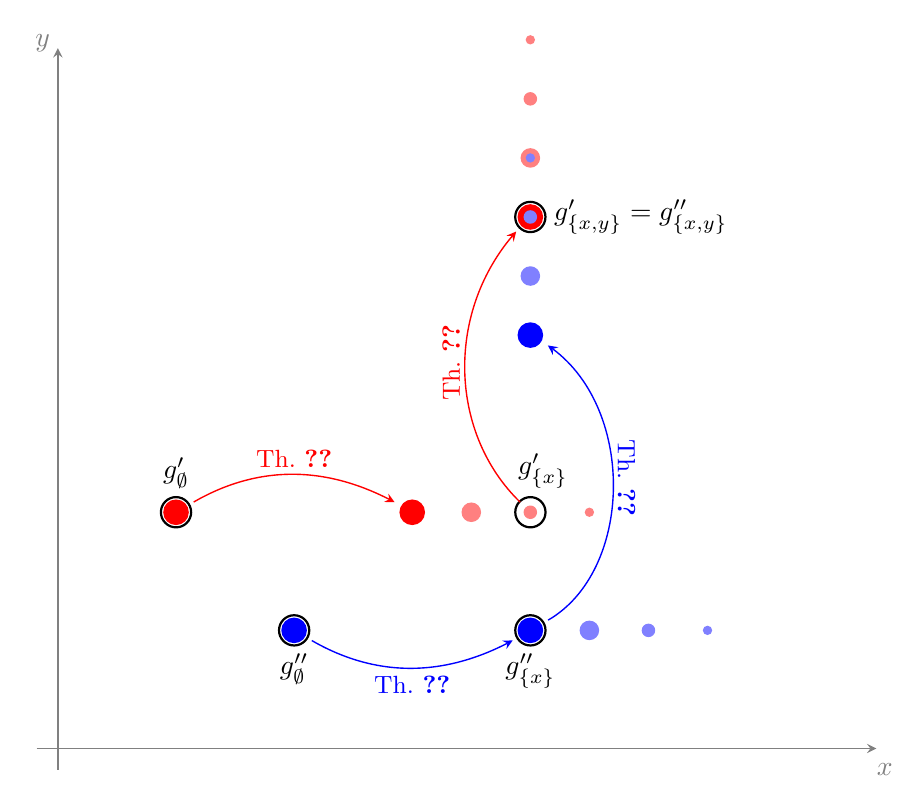
\begin{tikzpicture}[scale=1.5]
\tikzstyle{dot} = [draw, shape=circle, fill, minimum size=2mm, inner sep=0pt, outer sep=0pt]
\tikzstyle{circle} = [draw, thick, shape=circle, minimum size=2mm, inner sep=0pt, outer sep=0pt]
\tikzstyle{arrow} = [->, >=stealth, shorten >=1pt]
\path [gray, arrow] (-0.25,0) edge (7,0);
\path [gray, arrow] (0,-0.25) edge (0,6);
\path [gray, arrow] (7, 0) node [below = 1mm] {$\formal x$};
\path [gray, arrow] (0,6) node [left = 1mm] {$\formal y$};

\node [dot, red] (x') at (1,2) {};
\node [dot, blue] (x'') at (2,1) {};
\node [dot, red] (y') at (3,2) {};
\node [dot, red!50, scale=0.75] at (3.5,2) {};
\node [dot, red!50, scale=0.5] (y'bis) at (4,2) {};
\node [dot, red!50, scale=0.325] at (4.5,2) {};
\node [dot, blue] (y'') at (4,1) {};
\node [dot, blue!50, scale=0.75] at (4.5,1) {};
\node [dot, blue!50, scale=0.5] at (5,1) {};
\node [dot, blue!50, scale=0.325] at (5.5,1) {};
\node [dot, red] (z') at (4,4.5) {};
\node [dot, red!50, scale=0.75] at (4,5) {};
\node [dot, red!50, scale=0.5] at (4,5.5) {};
\node [dot, red!50, scale=0.325] at (4,6) {};
\node [dot, blue] (z'') at (4,3.5) {};
\node [dot, blue!50, scale=0.75] at (4,4) {};
\node [dot, blue!50, scale=0.5] at (4,4.5) {};
\node [dot, blue!50, scale=0.325] at (4,5) {};

\node [circle, black, scale=1.25] at (x') {};
\node [circle, black, scale=1.25] at (x'') {};
\node [circle, black, scale=1.25] at (y'bis) {};
\node [circle, black, scale=1.25] at (y'') {};
\node [circle, black, scale=1.25] (z) at (4,4.5) {};

\node [above=3mm] at (x') {$g'_{\emptyset}$};
\node [below=3mm] at (x'') {$g''_{\emptyset}$};
\node [above=3mm] at (y'bis) {$\phantom{X}g'_{\{\formal x\}}$};
\node [below=3mm] at (y'') {$g''_{\{\formal x\}}$};
\node [right=3mm] at (z) {$g'_{\{\formal x,\formal y\}} = g''_{\{\formal x,\formal y\}}$};

\path [red, arrow] (x') edge [bend left] node [above=0.2mm, red] {\small Th.~\ref{thm:saarela}} (y');
\path [blue, arrow] (x'') edge [bend right] node [below=0.8mm, blue] {\small Th.~\ref{thm:saarela}} (y'');
\path [red, arrow] (y'bis) edge [bend left=45] node [above=0.6mm, red, rotate=90] {\small Th.~\ref{thm:saarela}} (z');
\path [blue, arrow] (y'') edge [bend right=60] node [above=0.6mm, blue, rotate=-90] {\small Th.~\ref{thm:saarela}} (z'');
\end{tikzpicture}
\caption{Illustration of an argument for the proof of Corollary \ref{cor:saarela1}}\label{fig:saarela1}
\end{figure}

\begin{proof}
All inequalities considered hereafter have 
parameters in $\formal X=\{\formal{x}_1,\dots,\formal{x}_k\}$.
We are going to compare functions from $\formal X$ to $\mathbb{N}$
based on suitable partial orders, each parametrized by a variable. 
\AP
Formally, given two functions $f,g:\formal X\rightarrow\mathbb{N}$
and a variable $\formal x\in\formal X$, we write 
$f \mathrel{\plex*{\formal x}} g$ 
iff $f(\formal x) \le g(\formal x)$ and $f(\formal y) = g(\formal y)$ 
for all $\formal y\in\formal X\setminus\{\formal x\}$.
We prove the following two properties (the first property is equivalent to 
the claim of the lemma):
\begin{align}
  &\bigwedge_{e\in E}
    \exists f \in \sol{e}
    ~~\rightarrow~~
   \exists g \in \sol{E}
  \label{eq:exists-solution}
  \\
  &\forall f \in \sol{E} ~~
  \forall \formal x\in\formal X ~~
  \exists g \pgex{\formal x} f ~~
  \forall h \pgex{\formal x} g ~~:~~
  h \in \sol{E} 
  \label{eq:forall-solutions}
\end{align}
The proof goes by  double induction on the cardinality of $E$ 
and the number $k$ of parameters.

The base case is when $E$ has cardinality $1$.
In this case Property \eqref{eq:exists-solution} holds trivially.
We see how Property \eqref{eq:forall-solutions} follows from Theorem~\ref{thm:saarela}.
Let $E=\{e\}$, $f\in\sol{e}$, and fix an arbitrary variable $\formal x\in\formal X$.
We construct the inequality $e'$ with $\formal x$ as single formal parameter, by 
instantiating in $e$ every other parameter $\formal y\in\formal X\setminus\{\formal x\}$
with the value $f(\formal y)$. 
By construction, $f$ restricted to $\{\formal x\}$ is a solution of $e'$, and thus, 
by Theorem \ref{thm:saarela}, $\sol{e'}$ is co-finite. 
This means that there is a number $x_0\in\mathbb{N}$ such that $x_0 \ge f(\formal x)$ 
and, for all $x_1 \ge x_0$, the mapping $\formal x\mapsto x_1$ is a solution to $e'$ as well.
This property can be transferred to the original inequality $e$, as follows.
We define $g = f[\formal x / x_1]$ as the function obtained from $f$ by replacing
the image of $\formal x$ with $x_1$. Note that $g \ge_{\formal x} f$ and,
for all $h \pgex{\formal x} g$, $h\in\sol{e}$. This proves Property \eqref{eq:forall-solutions}.

As for the inductive step, suppose that $E$ is a system with at least two inequalities,
and divide $E$ into two sub-systems, $E'$ and $E''$, with cardinalities strictly 
smaller than that of $E$.

Let us first prove Property \eqref{eq:exists-solution} for $E$.
Suppose that every inequality in $E$ is satisfiable.
By the inductive hypothesis, $E'$ and $E''$ are also satisfiable;
in particular, there exist solutions $g'$ and $g''$ of $E'$ and $E''$, respectively.
We proceed with a second induction to prove that, for larger and larger
sets of variables $\formal Y\subseteq\formal X$, there are solutions
of $E'$ and $E''$ that agree on all the variables from $\formal Y$, namely:
\begin{align*}
  \exists g'_{\formal Y}\in\sol{E'} ~~
  \exists g''_{\formal Y}\in\sol{E''} ~~
  \forall \formal y\in \formal Y ~~
  g'_{\formal Y}(\formal y) = g''_{\formal Y}(\formal y) \ .
  \tag{$\star$}
\end{align*}
Of course, for $\formal Y=\formal X$, the above property will imply 
the existence of a solution of $E$.
The reader can refer to Figure \ref{fig:saarela1} as an illustration 
of the arguments that follow (axes correspond to variables, and red 
and blue dots represent solutions of the systems $E'$ and $E''$,
respectively).

For $\formal Y=\emptyset$, the claim ($\star$) is trivial, 
since we can simply let $g'_\emptyset = g'$ and $g''_\emptyset = g''$.
For the inductive step, suppose that ($\star$) holds for $\formal Y$
and let us prove it also holds for $\formal Y' = \formal Y \uplus \{\formal x\}$. 
By inductive hypothesis, $E'$ and $E''$ satisfy Property \eqref{eq:forall-solutions}.
In particular, by instantiating $f$ with $g'_{\formal Y}$ (resp.~$g''_{\formal Y}$)
in Property \eqref{eq:forall-solutions}, 
we obtain the existence of $g' \pgex{\formal x} g'_{\formal Y}$ such that, 
for all $h' \pgex{\formal x} g'$, $h'\in\sol{E'}$
(resp.~$g'' \pgex{\formal x} g''_{\formal Y}$ such that, 
for all $h'' \pgex{\formal x} g''$, $h''\in\sol{E''}$). 
Note that the functions $g'_{\formal Y}$, $g''_{\formal Y}$, $g'$, $g''$ 
all agree on the variables from $\formal Y$.
Moreover, without loss of generality, we can assume that $g'$ and $g''$ also agree
on the variable $\formal x$: indeed, if this were not the case, we could simply 
replace the $\formal x$-images of $g'$ and $g''$ with $\max\{g'(\formal x),g''(\formal x)\}$,
without affecting the previous properties.
Property ($\star$) now follows from letting $g'_{\formal Y'} = g'$ and $g''_{\formal Y'} = g''$.
This concludes the proof of the inductive step for Property \eqref{eq:exists-solution}.

Let us now prove the inductive step for Property \eqref{eq:forall-solutions}.
Let $f$ be a solution of $E$ and let $\formal x\in\formal X$.
Since both $E'$ and $E''$ satisfy Property \eqref{eq:forall-solutions} 
and since $f\in\sol{E'} \cap \sol{E''}$, there are 
$g',g'' \pgex{\formal x} f$ such that, 
for all $h' \pgex{\formal x} g'$ and $h'' \pgex{\formal x} g''$,
$h'\in\sol{E'}$ and $h''\in\sol{E''}$.
Since $g',g'' \pgex{\formal x} f$, 
$g'$ and $g''$ agree on all variables, except possibly $\formal x$.
Without loss of generality, we can also assume that $g'$ and $g''$ 
agree on $\formal x$: as before, if this were not the case, 
we could replace the $\formal x$-images of $g'$ and $g''$ with 
$\max\{g'(\formal x),g''(\formal x)\}$, while preserving the previous properties. 
Now that we have $g'=g''$, we can use this function to witness
Property \eqref{eq:forall-solutions}, since, for all $h \pgex{\formal x} g'$ ($ = g''$),
we have $h\in \sol{E'} \cap \sol{E''} = \sol{E}$.
\end{proof}



The second corollary is related to the existence of large sets of 
solutions for a satisfiable word inequality that avoid any 
correlation between variables. 
To formalize the statement, it is convenient to fix a total order 
on the variables of the inequality, 
say~$\formal x_1,\dots,\formal x_k$,
and then identify every function $f:\formal X\rightarrow\mathbb{N}$ 
with the $k$-tuple of values $\bar x = (x_1,\dots,x_k)$, where 
$x_i = f(\formal x_i)$ for all $i=1,\dots,k$.
According to this correspondence, the corollary states the existence 
of sets of solutions that look like Cartesian products of finite
intervals of values, each with arbitrarily large cardinality.
The statement of the corollary is in fact slightly more complicated 
than this, as it discloses dependencies between the intervals.
We also observe that the order in which we list the variables 
is arbitrary, but different orders will induce different 
dependencies between intervals.


\begin{corollary}\label{cor:saarela2}
Let $e$ be a word inequality with repetitions parametrized in 
$\formal X = \{\formal x_1,\dots,\formal x_k\}$.
If $e$ is satisfiable, then 
\begin{align*}
  & \exists \ell_1 ~ \forall h_1 ~ \dots ~ \exists \ell_k ~ \forall h_k \\
  & \quad
  \underbrace{[\ell_1,h_1]}_{\text{values for }\formal x_1}
  \times \, \dots \, \times
  \underbrace{[\ell_k,h_k]}_{\text{values for }\formal x_k} 
  \subseteq~ \sol{e}.
\end{align*}
\end{corollary}

\begin{figure}[t]
\centering
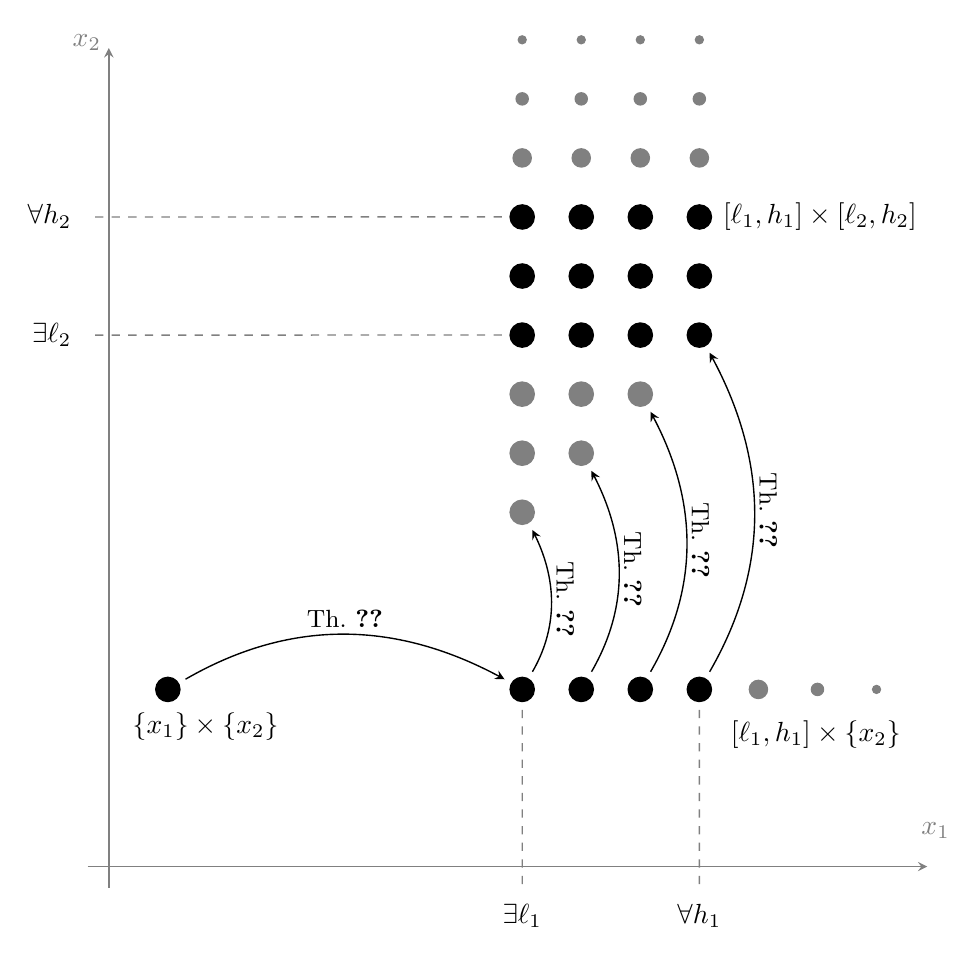
\begin{tikzpicture}[scale=1.5]
\tikzstyle{dot} = [draw, shape=circle, fill, minimum size=2mm, inner sep=0pt, outer sep=0pt]
\tikzstyle{circle} = [draw, thick, shape=circle, minimum size=2mm, inner sep=0pt, outer sep=0pt]
\tikzstyle{arrow} = [->, >=stealth, shorten >=1pt]
\path [gray, arrow] (-0.25,-0.5) edge (7,-0.5);
\path [gray, arrow] (0,-0.75) edge (0,6.5);
\path [gray, arrow] (7, 0) node [below = 1mm] {$\formal x_1$};
\path [gray, arrow] (0,6.5) node [left = 1mm] {$\formal x_2$};

\node [dot, black] (x) at (0.5,1) {};

\node [below=3mm] at (x) {$\phantom{XXX}\{x_1\}\times\{x_2\}$};

\node [dot, black!100, scale=1.0] (y1) at (3.5,1) {};
\node [dot, black!100, scale=1.0] (y2) at (4,1) {};
\node [dot, black!100, scale=1.0] (y3) at (4.5,1) {};
\node [dot, black!100, scale=1.0] (y4) at (5,1) {};
\node [dot, black!50, scale=0.75] (y5) at (5.5,1) {};
\node [dot, black!50, scale=0.5] (y6) at (6,1) {};
\node [dot, black!50, scale=0.325] (y7) at (6.5,1) {};

\path [gray, dashed] (y1) edge (3.5,-0.75);
\path [gray, dashed] (y4) edge (5,-0.75);
\path [black] (3.5,-0.75) node [below = 1mm] {$\exists\ell_1$};
\path [black] (5,-0.75) node [below = 1mm] {$\forall h_1$};

\node [below right=4mm] at (y4) {$[\ell_1,h_1]\times\{x_2\}$};

\node [dot, black!50, scale=1.0] (z11) at (3.5,2.5) {};
\node [dot, black!50, scale=1.0] (z12) at (3.5,3) {};
\node [dot, black!50, scale=1.0] (z13) at (3.5,3.5) {};
\node [dot, black!100, scale=1.0] (z14) at (3.5,4) {};
\node [dot, black!100, scale=1.0] (z15) at (3.5,4.5) {};
\node [dot, black!100, scale=1.0] (z16) at (3.5,5) {};
\node [dot, black!50, scale=0.75] (z17) at (3.5,5.5) {};
\node [dot, black!50, scale=0.5] (z18) at (3.5,6) {};
\node [dot, black!50, scale=0.325] (z19) at (3.5,6.5) {};

\node [dot, black!50, scale=1.0] (z21) at (4,3) {};
\node [dot, black!50, scale=1.0] (z22) at (4,3.5) {};
\node [dot, black!100, scale=1.0] (z23) at (4,4) {};
\node [dot, black!100, scale=1.0] (z24) at (4,4.5) {};
\node [dot, black!100, scale=1.0] (z25) at (4,5) {};
\node [dot, black!50, scale=0.75] (z26) at (4,5.5) {};
\node [dot, black!50, scale=0.5] (z27) at (4,6) {};
\node [dot, black!50, scale=0.325] (z28) at (4,6.5) {};

\node [dot, black!50, scale=1.0] (z31) at (4.5,3.5) {};
\node [dot, black!100, scale=1.0] (z32) at (4.5,4) {};
\node [dot, black!100, scale=1.0] (z33) at (4.5,4.5) {};
\node [dot, black!100, scale=1.0] (z34) at (4.5,5) {};
\node [dot, black!50, scale=0.75] (z35) at (4.5,5.5) {};
\node [dot, black!50, scale=0.5] (z36) at (4.5,6) {};
\node [dot, black!50, scale=0.325] (z37) at (4.5,6.5) {};

\node [dot, black!100, scale=1.0] (z41) at (5,4) {};
\node [dot, black!100, scale=1.0] (z42) at (5,4.5) {};
\node [dot, black!100, scale=1.0] (z43) at (5,5) {};
\node [dot, black!50, scale=0.75] (z44) at (5,5.5) {};
\node [dot, black!50, scale=0.5] (z45) at (5,6) {};
\node [dot, black!50, scale=0.325] (z46) at (5,6.5) {};

\path [gray, dashed] (z14) edge (-0.25,4);
\path [gray, dashed] (z16) edge (-0.25,5);
\path [black] (-0.25,4) node [left = 1mm] {$\exists \ell_2$};
\path [black] (-0.25,5) node [left = 1mm] {$\forall h_2$};

\node [right=3mm] at (z43) {$[\ell_1,h_1]\times[\ell_2,h_2]$};

\path [black, arrow] (x) edge [bend left] node [above=0.2mm] {\small Th.~\ref{thm:saarela}} (y1);
\path [black, arrow] (y1) edge [bend right] node [above=0.2mm, rotate=-90] {\small Th.~\ref{thm:saarela}} (z11);
\path [black, arrow] (y2) edge [bend right] node [above=0.2mm, rotate=-90] {\small Th.~\ref{thm:saarela}} (z21);
\path [black, arrow] (y3) edge [bend right] node [above=0.2mm, rotate=-90] {\small Th.~\ref{thm:saarela}} (z31);
\path [black, arrow] (y4) edge [bend right] node [above=0.2mm, rotate=-90] {\small Th.~\ref{thm:saarela}} (z41);
%\path [blue, arrow] (y'') edge [bend right=80] (z'');
\end{tikzpicture}
\caption{Illustration of an argument for the proof of Corollary \ref{cor:saarela2}}\label{fig:saarela2}
\end{figure}

\begin{proof}
Let $e$ be a satisfiable word inequality parametrized in $\formal X$ and
let $\bar x = (x_1,\dots,x_k)$ be any solution of $e$.
We will prove the following claim by induction on $i=0,\dots,k$:
\begin{align*}
 & \exists \ell_1 ~ \forall h_1 ~ \dots ~ \exists ~ \ell_i ~ \forall h_i\\
 & \quad
 [\ell_1,h_1]\times\cdots\times[\ell_i,h_i]\times\{x_{i+1}\}\times\dots\times\{x_k\} \subseteq \sol{e}
 \tag{$\star$}
\end{align*}
Note that for $i=k$ the above claim coincides with the statement of the corollary.
The reader can also refer to Figure \ref{fig:saarela2} as an illustration 
of the arguments that follow (axes correspond to variables $\formal x_1$ 
and $\formal x_2$, dots represent generic solutions of $e$, 
clusters of black dots represent solutions in the form of Cartesian products,
like those that appear in ($\star$).

For the base case $i=0$, the claim ($\star$) is vacuously true, as $\bar x=(x_1,\dots,x_k)$
is a solution of $e$.

For the inductive step, we need to show that 
if ($\star$) holds for $i<k$, then it also holds for $i+1$.
It is in fact sufficient to prove that, for $i<k$,
\[
  [\ell_1,h_1]\times\cdots\times[\ell_i,h_i]\times
  \{x_{i+1}\}\times\dots\times\{x_k\} 
  \subseteq \sol{e}
\]
implies
\begin{align*}
  & \exists \ell_{i+1} ~ \forall h_{i+1} \\
  & [\ell_1,h_1]\times\cdots\times[\ell_{i+1},h_{i+1}]\times
    \{x_{i+2}\}\times\dots\times\{x_k\} 
    \subseteq \sol{e}.
\end{align*}
%For this, it is convenient to think of the prefix of quantifiers in ($\star$) as a game, 
%where a player, say Eve, choses the existentially quantified values $\ell_i$, and an opponent, 
%say Adam, choses the universally quantified values $h_i$. 
%The fact that ($\star$) holds, means that Eve has strategy that, after $i$ rounds,
%no matter how Adam plays, always witnesses the containment
%$[\ell_1,h_1]\times\cdots\times[\ell_i,h_i]\times\{x_{i+1}\}\times\dots\times\{x_k\} \subseteq \sol{e}$.
%We rely on this assumed strategy to construct a strategy for Eve in the analogous game with $i+1$ rounds.
%In the first $i$ rounds Eve will play exactly as her strategy suggests for the $i$-round game.
%After Adam has chosen his last-but-one value $h_i$, the next value $\ell_{i+1}$ chosen by Eve is
%defined as follows.
For brevity, we let 
$S = [\ell_1,h_1]\times\dots\times[\ell_i,h_i]\times    
     \{x_{i+1}\}\times\dots\times\{x_k\}$,
and we assume that $S\subseteq \sol{e}$.
%be the set of tuples induced by the play so far.
For every tuple $\bar s\in S$, we consider the word inequality 
$e_{\bar s}$ over a single
variable $\formal x_{i+1}$ that is obtained from $e$ by instantiating every other variable
$\formal x_j$ ($j\neq i$) with $\bar s[j]$.
Since $S\subseteq\sol{e}$, we know that $e_{\bar y}$ is satisfiable, and hence
by Theorem \ref{thm:saarela}, $e_{\bar s}$ has co-finitely many solutions.
This means that there is $\ell_{\bar s}$ such that, for all $x'\ge \ell_{\bar s}$, 
$x'$ is also a solution of $e_{\bar s}$.
This property can be transferred to our original inequality $e$:

\begin{claim*}\label{claim:saarela3}
For every $\bar s\in S$, there is $\ell_{\bar s}$ such that,
for every $x'\ge \ell_{\bar s}$, the tuple $\bar s[i+1 \mapsto x']$, 
obtained from $\bar s$ by replacing the $(i+1)$-th value with $x'$,
is a solution of $e$.
\end{claim*}

Now, 
%at round $i+1$, the strategy of Eve is to choose 
the existentially quantified value $\ell_{i+1}$ 
can be set to
the maximum of the $\ell_{\bar s}$'s, for all $\bar s\in S$
(for this definition to make sense, it is crucial that the set $S$ is finite).
In this way, thanks to the previous claim, the containment 
$[\ell_1,h_1]\times\cdots\times[\ell_{i+1},h_{i+1}]\times\{x_{i+2}\}\times\dots\times\{x_k\} \subseteq \sol{e}$
holds for all choices of the universally quantified value $h_{i+1}$.
This proves the inductive step for $(\star)$ from $i$ to $i+1$.
\end{proof}

\subsection{Delay between accepting runs}\label{subsec:delay}

We briefly recall the definitions from \cite{SSTdelay}, that introduces
a measure of similarity (called delay)
between accepting runs of an SST that have the same input and the same output.

We first give some intuition, followed by definitions and an example.
%, see Example~\ref{ex:delay}.
Naturally, the difference between the amount of output symbols produced during a run should be an indicator of (dis)similarity. 
However, as SSTs do not necessarily build their output 
from left to right, one must also take into account 
the position where an output symbol is placed.
For example, compare two runs $\rho$ and $\rho'$ 
on the same input that produce the same output 
$aaabbb$. %$abcbca$. 
After consuming a prefix of the input, 
$\rho$ may have produced 
%$abc\_\ \_\ \_$ 
$aaa\_\ \_\ \_$ 
and $\rho'$ may have produced 
%$\_\ \_\ \_bca$. 
$\_\ \_\ \_bbb$. 
The amount of produced output symbols is the same,
but the runs are delayed because $\rho$ 
built the output from the left, 
whereas $\rho'$ did it from the right.
This idea of delay comes with an important caveat.
As another example, consider two runs $\rho$ and $\rho'$ 
on the same input that produce the same output 
%$abcabc$ 
$aaaaaa$,
and assume that, after consuming the same prefix of the input,
$\rho$ and $\rho'$ produced 
%$abc\_\ \_\ \_$ and $\_\ \_\ \_abc$, respectively. 
$aaa\_\ \_\ \_$ and $\_\ \_\ \_aaa$, respectively. 
Note that the output 
%$abcabc$ is a periodic word with primitive root $abc$.
$aaaaaa$ is a periodic word. %with primitive root $a$.
Hence, it does not matter if 
%$abc$ is appended or prepended to $abc$ 
$aaa$ is appended or prepended to a word with period $a$. % the current output 
% as long as the operations commute.
%in order to build the final output.
In general, one copes with this phenomenon 
by dividing the output into periodic parts,
where all periods are bounded by a well-chosen parameter $C$.
%(in the small examples above, we assume $C=3$). 
So, intuitively, the delay measures 
the difference between the numbers of output symbols that have 
been produced by the two runs, up to the end of each of periodic factor. The number of produced output symbols is formally captured 
by a weight function, defined below, and the delay aggregates
the weight differences. 

\AP
For an
accepting run $\rho$, a position $t$ of $\rho$, 
and a position $j$ in the output $\out{\rho}$, we denote by
$\weight*[t][j]{\rho}$ %
% \[
  % \weight*[t][j]{\rho}
% \]
the number of output positions $j'\le j$ that are produced by 
the prefix of $\rho$ up to position $t$.
%and have origin inside $I$.
%(the output profix $v$ is in fact a word \emph{annotated} 
%with the origns generated by $\rho$),
%\item \AP
%      $\diff*[\rho,\rho']{t,v} =
%       \weight[\rho]{t,v} - \weight[\rho']{t,v}$.
%\end{itemize}
We use the above notation when $j$ witnesses
a change in a repeating pattern of the output. These changes in repeating patterns are called cuts, as formalized below.

Let $w$ be any non-empty word (e.g.~the output of $\rho$ or a factor of it).
\AP
The \reintro{primitive root} of $w$, denoted $\rt*{w}$, 
is the shortest word $r$ such that $w \in \{r\}^*$.
% The \reintro{period} of $w$, denoted 
% $\period*{w}$, is the smallest number $n\ge 1$ such that 
% $w=w[1,n]^{\frac{|w|}{n}}$ (possibly
% $n=|w|$).\anca{usually this is not the period, but the root}
\AP
For a fixed integer $C>0$ we define a factorization 
$w[1,j_1],w[j_1+1,j_2],\dots,w[j_n + 1,j_{n+1}]$
of $w$ in which every $j_i$ is chosen as the rightmost 
position for which $w[j_{i-1}+1, j_i]$ has primitive root 
of length not exceeding $C$.
These positions $j_1,\dots,j_n$ are called $C$-cuts.
More precisely:
\begin{itemize}
\item the \reintro[$C$-cuts]{first $C$-cut} of $w$ is the largest position $j\le |w|$, 
      such that $|\rt{w[1,j]}| \le C$;
\item if $j$ is the $i$-th $C$-cut of $w$,
      then the  \reintro[$C$-cuts]{$(i+1)$-th $C$-cut} of $w$ 
      is the largest position $j'>j$ such that 
      $|\rt{w[j+1,j']}| \le C$.
\end{itemize}
\AP
We denote by $\cuts*<C>{w}$ 
the set of all $C$-cuts of $w$.

\AP
We are now ready to define the notion of delay.
Consider two accepting runs $\rho,\rho'$ of an SST 
with the \emph{same input} $u=\inp{\rho}=\inp{\rho'}$ and the 
\emph{same output} $w=\out{\rho}=\out{\rho'}$,
and define:
\[
  \delay*<C>{\rho,\rho'} ~= 
  \max\limits_{\substack{t\le |u|, \\ j\,\in\,\cuts{w}}} ~ 
  \big| \weight[t][j]{\rho} - \weight[t][j]{\rho'} \big|
\]
In other words, the delay between two such runs $\rho$ and $\rho'$ measures over all input positions the maximal difference between the amount of generated output, but only up to $C$-cuts  of the output.
Note that the delay is only defined for accepting runs with 
same input and output. 
So whenever we write $\delay<C>{\rho,\rho'}$, we implicitly mean 
that $\rho,\rho'$ have \emph{same input and same output}.


\begin{example}\label{ex:delay}
Let $w = abcccbb$ be the output of runs $\rho, \rho'$ 
on the same input of length $2$. 
Assume $\rho$ produces $abc\_\ \_bb$ and then $abcccbb$, 
whereas $\rho'$ produces $\_\ \_\ \_c\_bb$ and then $abcccbb$.
For $C = 2$, we obtain $\cuts<2>{w} = \{2,5,7\}$, i.e., $w$ is divided into $ab|ccc|bb$.
To compute the $\delay<2>{\rho,\rho'}$, we need to calculate weights
at cuts. For $t=0$, $\weight[0][j]{\rho} =
\weight[0][j]{\rho'} = 0$ for all $j\in \cuts<2>{w}$ because nothing
has been produced. For $t=2$, $\weight[2][j]{\rho} =
\weight[2][j]{\rho'} = j$ for all $j\in \cuts<2>{w}$ because the whole output
has been produced. Only the case $t=1$ has an impact on the delay. 
We have $\weight[1][2]{\rho} = 2$, $\weight[1][5]{\rho} = 3$, and $\weight[1][7]{\rho} = 5$.
Also, we have $\weight[1][2]{\rho'} = 0$, $\weight[1][5]{\rho} = 1$, and $\weight[1][7]{\rho} = 3$.
Hence, we obtain $\delay<2>{\rho,\rho'} = 2$. 
\end{example}

We recall below some crucial results obtained in \cite{SSTdelay}.
A first result shows that the relation of pairs of runs 
having bounded delay (for a fixed bound) is automatic
--- for this to make sense, we view a run of an SST
as a finite word, with letters representing transitions, 
and we recall that a relation is automatic 
if its convolution language is regular.


\begin{lemma}[{\cite[Theorem 5]{SSTdelay}}]\label{lem:regular-delay}
Given an SST and some numbers $C,D$, the relation consisting of
pairs of accepting runs $(\rho,\rho')$ such that $\delay<C>{\rho,\rho'} \le D$ 
is automatic.
\end{lemma}

\begin{proof}
The statement in \cite[Theorem 5]{SSTdelay} is not for runs of SSTs,
but for sequences of updates. One can easily build an automaton 
that checks if two sequences of transitions, encoded by their convolution,
form accepting runs $\rho,\rho'$ of the given SST on the same input. 
The remaining condition $\delay<C>{\rho,\rho'} \le D$ only depends on 
the underlying sequences of updates determined by $\rho$ and $\rho'$,
and can be checked using \cite[Theorem 5]{SSTdelay}.
\end{proof}


%\christof{Maybe we can say somewhere that the roles of $C$ and $k$ have switched compared to \cite[proof of Lemma 6]{SSTdelay}. $C,D$ here is $k,\ell$ there, and $k$ here is $C$ there.}
A second result shows that given two runs with large
delay, one can find a set of positions on the input 
(the cardinality of which depends on how large the delay is)
in such a way that any interval starting just before any of 
these positions and ending just after any other of these positions 
is a loop on both runs such that, when pumped, produces 
different outputs. 
Roughly, the reason for obtaining different outputs is that pumping creates a misalignment between $C$-cuts that were properly aligned before pumping, and different periods cannot overlap.
By this last result, large delay intuitively means 
``potentially different outputs''.


\begin{lemma}[name={\cite[Lemma 6]{SSTdelay}}]\label{lem:delay-vs-output}%
Given an SST, one can compute%
\footnote{%
We remark that the notation and the actual bounds here 
differ from the original presentation of \cite{SSTdelay},
mainly due to the fact that here we manipulate runs
with explicit states and loops with idempotent skeletons.
In particular, the parameters $C,D,m$ here correspond respectively to 
the values $k E^2, \ell E^4, C E^2$ with $k,\ell,C$ as in \cite[Lemma 6]{SSTdelay}, and
 $E$ as in our Lemma \ref{lem:ramsey}.
}
some numbers $C,D$ such that, 
for all $m\ge 1$ and all runs $\rho,\rho'$:
if $\delay<C m>{\rho,\rho'} > D m^2$,
then there exist
$m$ positions $0\le \ell_1 < \dots < \ell_m \le |\rho|$ such that,
for every $1 \le i < j \le m$, the interval $L_{i,j}=[\ell_i,\ell_j]$
is a loop on both $\rho$ and $\rho'$ and satisfies
\[
  \out{\pump<2>[L_{i,j}]{\rho}} 
  \:\neq\: 
  \out{\pump<2>[L_{i,j}]{\rho'}} .
\]
\end{lemma}

To reason about finite valuedness we will need to consider 
\emph{several} accepting runs on the same input, with pairwise 
large delays.
By Lemma \ref{lem:delay-vs-output}, 
every two such runs can be pumped so as to witness different outputs. 
The crux however is to show that these runs can be pumped \emph{simultaneously} 
so as to get pairwise different outputs.
This is indeed possible thanks to: 

\begin{lemma}\label{lem:saarela-delay}\label{cor:saarela-delay}
Let $C,D$ be computed as in Lemma \ref{lem:delay-vs-output},
%$E$ be computed as in Lemma \ref{lem:ramsey},
and $k$ be an arbitrary number. Then one can compute a number $m$
such that, for all runs $\rho_0,\dots,\rho_k$ on the same input and with 
$\displaystyle\bigwedge\nolimits_{0\le i<j\le k} 
 \big(\out{\rho_i} \neq \out{\rho_j} ~\vee~
      \delay<C m>{\rho_i,\rho_j} > D m^2\big)$,
there is a tuple 
$\bar{L} = (L_{i,j})_{0\le i<j\le k}$ of disjoint intervals
that are loops on all runs $\rho_0,\dots,\rho_k$,
and there is a tuple $\bar n = (n_{i,j})_{0\le i<j\le k}$
of positive numbers such that
\[
  \text{for all } 0\le i<j\le k\,, \quad 
  \out{\pump<\bar n>[\bar L]{\rho_i}} 
  \:\neq\:
  \out{\pump<\bar n>[\bar L]{\rho_j}} \, .
\]
\end{lemma} 
\begin{proof}
We first define $m$. % The idea is that we select, for a given pair of runs,
% $m$ intervals that are loops on both runs. 
% Then we want to select a subset of size $k(k+1)$ of these intervals that 
% are loops also on all other runs. We do this by $k-1$ applications of 
% Lemma~\ref{lem:ramsey}. 
Let $E,H$ be as in Lemma~\ref{lem:ramsey}, and set $m:=m_0+1$ for 
the sequence $m_0, \ldots, m_{k-1}$ defined inductively by 
$m_{k-1} := k(k+1)$, and 
%$m_i := E(m_{i+1}^H+1)$. 
$m_h := E m_{h+1}^H$. 

We show how to pump the runs in such a way that all pairs of indices $i<j$
witnessing $\delay<C m>{\rho_i,\rho_j} > D m^2$ before pumping,
will witness different outputs after pumping.
Consider one such pair $(i,j)$, with $i<j$, such that 
%  $\out{\rho_i} = \out{\rho_j}$ and
$\delay<C m>{\rho_i,\rho_j} > D m^2$, so in particular,
$\out{\rho_i} = \out{\rho_j}$
(if there is no such pair, then all runs have pairwise different
outputs, and so we are already done).
We apply Lemma \ref{lem:delay-vs-output}
and obtain a set $I_{i,j,0}$ of $m = m_0+1$ positions such that each interval $L=[\ell,\ell']$ with $\ell,\ell' \in I_{i,j,0}$ is a loop on both $\rho_i$ and $\rho_j$, and:
\begin{equation}\label{eq:divergence1}
  \out{\pump<2>[L]{\rho_i}} \neq \out{\pump<2>[L]{\rho_j}}.
\end{equation}
Then, by repeatedly using Lemma~\ref{lem:ramsey}, 
we derive the existence of sets $I_{i,j,k-1} \subseteq  \cdots \subseteq I_{i,j,1} \subseteq I_{i,j,0}$ with $|I_{i,j,h}| = m_h+1$ such that each interval $L=[\ell,\ell']$ with $\ell,\ell' \in I_{i,j,h}$ is a loop on $\rho_i,\rho_j$, and $h$ further runs from $\rho_0,\ldots,\rho_k$ (our definition of $m$ from the 
beginning of the proof is tailored to this repeated application
of Lemma~\ref{lem:ramsey}, because $|I_{i,j,h}| = m_h+1 = E m_{h+1}^H +1$). In particular, all intervals with endpoints in $I_{i,j,k-1}$ are loops on all the $\rho_0,\ldots,\rho_k$.

In this way, for each pair $i<j$ such that $\rho_i$ and $\rho_j$ 
have large delay, we obtain $k(k+1)$ adjacent intervals that are loops on all runs and that satisfy the pumping property (\ref{eq:divergence1}) from above.

As there are at most $k (k+1)$ pairs of runs, 
we can now choose from the sets of intervals that we have prepared 
one interval $L_{i,j}$ for each pair $i<j$ with $\delay<C m>{\rho_i,\rho_j} > D m^2$,
in such a way that all the chosen intervals are pairwise disjoint 
(for example, we could do so by always picking among the remaining intervals 
the one with the left-most right border, and then removing all intervals 
that intersect this one).
The selected intervals $L_{i,j}$ thus have the following properties:
\begin{enumerate}
\item $L_{i,j}$ is a loop on all runs $\rho_0,\dots,\rho_k$,
\item $L_{i,j}$ is disjoint from every other interval $L_{i',j'}$,
\item $\out{\pump<2>[L_{i,j}]{\rho_i}} \neq \out{\pump<2>[L_{i,j}]{\rho_j}}$.
\end{enumerate}
%
If a pair $i<j$ of runs is such that 
$\out{\rho_i} \neq \out{\rho_j}$, 
then we set $L_{i,j}$ as an empty loop. 
% arbitrary loop on all
% runs $\rho_0,\dots,\rho_k$, that is disjoint from all other intervals
% $L_{i',j'}$.
%Note that in this case $\out{\pump<1>[L_{i,j}]{\rho_i}} \neq \out{\pump<1>[L_{i,j}]{\rho_j}}$.

Now, let $\bar{L} = (L_{i,j})_{0 \le i < j \le k}$ be the tuple of chosen intervals, and consider the following system of word inequalities with formal parameters $(\formal{x}_{i,j})_{0\le i < j \le k} =: \bar{\formal{x}}$:
\[
  \text{for all } 0\le i<j\le k\,, \quad 
  \out{\pump<\bar{\formal{x}}>[\bar L]{\rho_i}} 
  \:\neq\:
  \out{\pump<\bar{\formal{x}}>[\bar L]{\rho_j}} \, .
\]
Here, the value of the formal parameter $\formal{x}_{i,j}$ determines how often the loop $L_{i,j}$ is pumped. By Corollary \ref{cor:loop-pumping}, this corresponds to a word inequality in the parameters $\formal{x}_{i,j}$.

Note that there is one such inequality for each pair of runs $\rho_i,\rho_j$ with $0 \le i < j \le k$. 
By the choice of the intervals in $\bar{L}$, each of the inequalities is satisfiable: 
indeed, the inequality for $\rho_i,\rho_j$ is satisfied by letting 
$\formal{x}_{i',j'} = 1$ if $i' \not = i$ or $j' \not = j$, and
$\formal{x}_{i,j} = 2$ otherwise. 

By Corollary~\ref{cor:saarela1}, the system of inequalities is also satisfiable with a tuple $\bar n = (n_{i,j})_{0 \le i < j \le k}$ of numbers, as claimed in the lemma.
\end{proof}





\section{The Decomposition Theorem}\label{sec:decomposition}


This section is devoted to the proof of the Decomposition Theorem:
\RestateGo{\restateDecomposition}
\Decomposition*

 
Our proof relies on the notion of 
\emph{cover} of an SST, which is
reminiscent of the so-called ``lag-separation covering''
construction \cite{deSouza-thesis,SakarovitchDeSouzaMFCS08}.
Intuitively, given an SST $T$ and 
two integers $C,D \in \mathbb{N}$,
%we use the notion of $C$-delay
%to prune some runs of $T$ and 
we construct an SST $\Cover{T}$
that is equivalent to $T$,
yet for each input $u$ it only admits 
pairs of accepting runs with 
different outputs or $C$-delay larger than $D$. 
The crucial point will be that $\Cover{T}$ is $k$-ambiguous when $T$ is $k$-valued. 



\begin{proposition}\label{prop:separation-covering}
Given an SST $T$ and two numbers $C,D$, 
one can compute an SST called
$\Cover*[C,D]{T}$ such that
\begin{enumerate}
\item $\Cover{T}$ is equivalent to $T$;
\item for every two accepting runs $\rho\neq\rho'$ of $\Cover{T}$ 
      having the same input, 
      either $\out{\rho} \neq \out{\rho'}$ or $\delay<C>{\rho,\rho'} >~D$;
\item every accepting run of $\Cover{T}$ can be projected onto an accepting run of $T$.
\end{enumerate}
\end{proposition}

\begin{proof}
We order the set of accepting runs of $T$ lexicographically,
and we get rid of all the runs for which there exists a 
lexicographically smaller run with the same input, 
the same output, and small delay. 
Since all these conditions are encoded by regular languages, 
the remaining set of runs is also regular, and this can be 
used to construct an SST $\Cover{T}$ that satisfies the 
required properties.

We now give more details about this construction. 
Let $R$ denote the set of all accepting runs of $T$.
Remark that $R$ is a language over the alphabet consisting 
of transitions of $T$, and it is recognized by the underlying 
automaton of $T$, so it is regular.
\AP
Let
\[
    \Sep*{R}
    ~=~
        \big\{  \rho \in R
                ~\big|~
			    \nexists \rho' \in R \; .\,
			    \rho' \!<\! \rho ~\wedge~ \delay<C>{\rho,\rho'} \leq D
        \big\}.
\]
Recall that the delay is only defined for accepting runs 
with same input and same output, 
so $\delay<C>{\rho,\rho'} \leq D$ implies that $\inp{\rho} = \inp{\rho'}$ 
and $\out{\rho} = \out{\rho'}$.
We show that
\begin{enumerate}[label={\sc\alph*)}]
    \item \label{item:sep1}
          $\Sep{R}$ is a regular subset of $R$;
    \item \label{item:sep2}
          $\{(\inp{\rho}, \out{\rho}) \:\mid\: \rho \in \Sep{R}\} = \{(\inp{\rho}, \out{\rho}) \:\mid\: \rho \in R\}$;
    \item \label{item:sep3}
          for every pair of runs $\rho, \rho' \in \Sep{R}$ over the same input,
          either $\out{\rho} \neq \out{\rho'}$ or $\delay<C>{\rho,\rho'} > D$.
\end{enumerate}
Before proving these properties, let us show how to use them to conclude the 
proof of the proposition:

We start with a DFA $A$ recognizing $\Sep{R}$, whose existence is guaranteed by 
Property \ref{item:sep1}. Note that the transitions of $A$ are of the form
$\big(q,(s,a,\alpha,s'),q'\big)$, where $(s,a,\alpha,s')$ is a transition of $T$.
Without loss of generality, we assume that the source state $q$ 
of an $A$-transition determines the source state $s$ 
of the corresponding $T$-transition, and similarly
for the target states $q'$ and $s'$.
Thanks to this, we can turn $A$ into the desired SST $\Cover{T}$
by simply projecting away 
the $T$-states from the $T$-transitions, namely, by replacing every transition
$\big(q,(s,a,\alpha,s'),q'\big)$ with $(q,a,\alpha,q')$. 
To complete the construction, we observe that if the state $q'$
is final in $A$, then the corresponding state $s'$ is also final in $T$
(this is because $A$ recognizes only accepting runs of $T$). 
Accordingly, we can define the final update of $\Cover{T}$
so that it maps any final state $q'$ of $A$ to the 
final update $\finalupd(s')$, as determined by the corresponding
final state $s'$ in $T$.
Finally, thanks to Properties \ref{item:sep2} and \ref{item:sep3}, 
the SST $\Cover{T}$ constructed in this way clearly satisfies the 
properties claimed in the proposition.

Let us now prove Properties \ref{item:sep1}--\ref{item:sep3}.


\smallskip\noindent
{\sc Proof of Property \ref{item:sep1}.}~
Note that the set $\Sep{R}$ is obtained 
by combining the relations $R$, 
$\{ (\rho,\rho') ~|~ \rho' < \rho\}$, and
$\{ (\rho,\rho') ~|~ \delay<C>{\rho,\rho'} \leq~D\}$ 
using the operations of intersection, projection, and complement.
Also recall that $R$ can be regarded a regular language, and that
$\{ (\rho,\rho') ~|~ \rho' < \rho\}$ and
$\{ (\rho,\rho') ~|~ \delay<C>{\rho,\rho'}~\leq ~D\}$
are automatic relations (for the latter one uses Lemma~\ref{lem:regular-delay}).
It is also a standard result (cf.~\cite{Hodgson83,KhoussainovN95,BlumensathG00})
that automatic relations are closed under intersection, projection, and
complement.
From this it follows that $\Sep{R}$ is a regular language.



\smallskip\noindent
{\sc Proof of Property \ref{item:sep2}.}~
%In order to prove that the two sets are equal, we show both inclusions.
As $\Sep{R} \subseteq R$, the left-to-right inclusion is immediate.
To prove the converse inclusion,
consider an input-output pair $(u,v)$ in the right hand-side of the equation,
namely, $(u,v)$ is a pair in the relation realized by $T$.
Let $\rho$ be the lexicographically least accepting run of $T$
such that $\inp{\rho}=u$ and $\out{\rho}=v$.
By construction, $\rho\in\Sep{R}$ and hence $(u,v)$ also belongs to the
left hand-side of the equation.


\smallskip\noindent
{\sc Proof of Property \ref{item:sep3}.}~
This holds trivially by the definition of $\Sep{R}$.
\end{proof}

We can now present the missing ingredients of the decomposition result.
Proposition \ref{prop:coveringIsFiniteValued} below
shows that, for suitable choices of $C$ and $D$
that depend on the valuedness of $T$, 
$\Cover{T}$ turns out to be $k$-ambiguous.

This will enable the decomposition result
via a classical technique that decomposes any 
$k$-ambiguous automaton/transducer into a 
union of $k$ unambiguous ones
(see Proposition \ref{prop:FiniteValuedToDecomposition}
further below). 


\begin{proposition}\label{prop:coveringIsFiniteValued}
Let $T$ be a $k$-valued SST and let $C,D,m$ be
as in Lemma~\ref{lem:saarela-delay} (note that $m$ depends on $k$).
The SST $\Cover[Cm,Dm^2]{T}$ is $k$-ambiguous.
\end{proposition}

\begin{proof}
We prove the contrapositive of the statement. Assume that 
$\Cover[Cm,Dm^2]{T}$ is not $k$-ambiguous, that is, 
it admits $k+1$ accepting runs $\rho_0, \dots, \rho_k$ 
on the same input. 
Recall from Proposition \ref{prop:separation-covering} 
that for all $0\le i<j\le k$, 
either $\out{\rho_i} \neq \out{\rho_j}$ or $\delay<Cm>{\rho_i,\rho_j} > Dm^2$.
By Lemma~\ref{lem:saarela-delay} we can find pumped versions
of the runs $\rho_0, \dots, \rho_k$ that have all the same input 
but have pairwise different outputs, and thus $T$ is not $k$-valued.
\end{proof}


\begin{proposition}\label{prop:FiniteValuedToDecomposition}
For all $k \in \mathbb{N}$, every $k$-ambiguous SST 
can be decomposed into a union of $k$ unambiguous SSTs.
\end{proposition}

\begin{proof}
The decomposition is done via a classical 
technique applicable to $k$-ambiguous NFA and, 
by extension, to all variants of automata and transducers
(see~\cite{JohnsonICALP85,Sakarovitch98}).
More precisely, decomposing a $k$-ambiguous NFA into a union of $k$ 
unambiguous NFA is done by ordering runs lexicographically 
and by letting the $i$-th NFA in the decomposition guess
the $i$-th accepting run on a given input (if it exists).
Since the lexicographic order is a regular property of pairs of runs,
it is easy to track all smaller runs.
\end{proof}


\paragraph{Proof of Theorem~\ref{thm:FiniteValuedToDecomposition}.} 
We now have all the ingredients to prove
Theorem~\ref{thm:FiniteValuedToDecomposition}, which directly
follows from Propositions~\ref{prop:coveringIsFiniteValued}
and~\ref{prop:FiniteValuedToDecomposition}, and the fact that
unambiguous SSTs can be determinized~\cite{DBLP:conf/fsttcs/AlurC10}. %\cite{DBLP:conf/icalp/AlurD11}.
\qed




\section{Finite valuedness}\label{sec:finite-valuedness}

We characterize finite valuedness of SSTs 
by excluding certain types of substructures.
Our characterization has strong analogies with 
the characterization
%s of boundedness for weighted transducers and 
of finite valuedness for one-way transducers,
where the excluded substructures have the shape 
of a ``W'' and are therefore called \emph{W-patterns} 
(cf.~\cite{deSouza-thesis}).%
\footnote{\cite{deSouza-thesis} 
          used also other excluded substructures,
          but they can be seen as degenerate cases 
          of W-patterns.}
          


\begin{definition}\label{def:W-pattern}
A W-pattern is a substructure of an SST 
consisting of states $q_1,q_2,r_1,r_2,r_3$,
and some initial and final states, that are 
connected by runs as in the diagram of Figure~\ref{fig:Wpattern}.
%\[
\begin{figure}[ht]
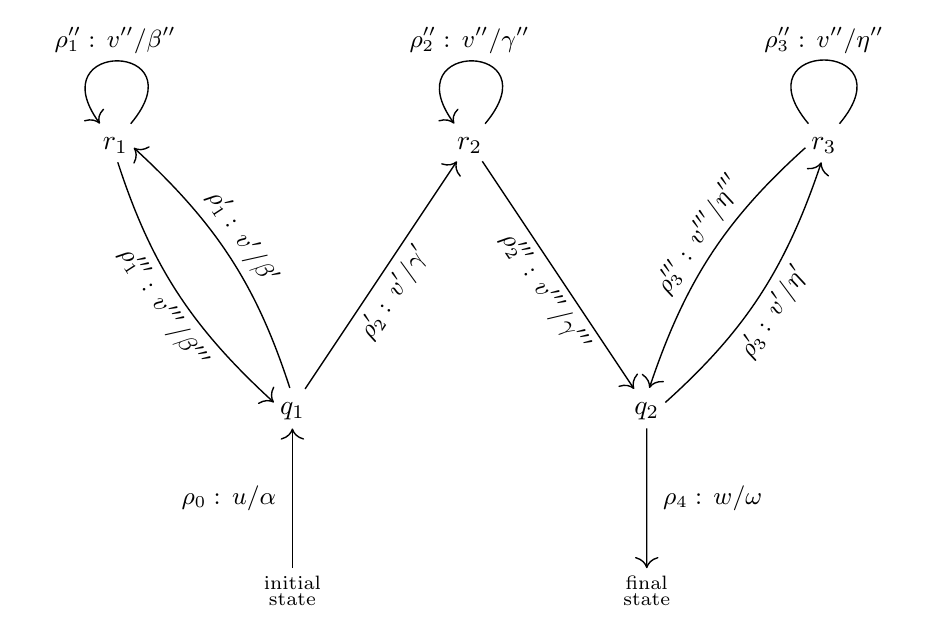
\begin{tikzpicture}[scale=1.5]
%\draw (-2.2,-0.2) rectangle (5.2,5.4);
%\myclip{-2.2,0}{5.2,5.4}
%
\node (q) at (0,1.75) {$q_1$};
\node (q') at (3,1.75) {$q_2$};
\node (r) at (-1.5,4) {$r_1$};
\node (s) at (1.5,4) {$r_2$};
\node (t) at (4.5,4) {$r_3$};
%
\node (initial) at (0,0.2) 
      {$\begin{subarray}{c} \text{initial} \\ \text{state} \end{subarray}$};
\node (final) at (3,0.2) 
      {$\begin{subarray}{c} \text{final} \\ \text{state} \end{subarray}$};
%
\draw (initial) edge [arrow] node [left=1mm] {\small $\rho_0:\, u/\alpha~$} (q);
\draw (q') edge [arrow] node [right=1mm] {\small $~\rho_4:\, w/\omega$} (final);
%
\draw (q.north) edge [arrow, bend right=15] 
      node [sloped, above=1mm] {\small $\rho'_1:\, v'/\beta'~~$} (r.east);
\draw (r) edge [arrow, loop above] 
      node [above=1mm] {\small $\rho''_1:\, v''/\beta''$} (r);
\draw (r.south) edge [arrow, bend right=15] 
      node [sloped, below=1mm] {\small $~\rho'''_1:\, v'''/\beta'''$} (q.west);
%
\draw (q) edge [arrow] 
      node [sloped, below=1mm] {\small $\rho'_2:\, v'/\gamma'\phantom{x}$} (s);
\draw (s) edge [arrow, loop above] 
      node [above=1mm] {\small $\rho''_2:\, v''/\gamma''$} (s);
\draw (s) edge [arrow] 
      node [sloped, below=1mm] {\small $\phantom{x}\rho'''_2:\, v'''/\gamma'''$} (q');
%
\draw (q'.east) edge [arrow, bend right=15] 
      node [sloped, below=1mm] {\small $\rho'_3:\, v'/\eta'~~$} (t.south);
\draw (t) edge [below, loop above] node [above=1mm] {\small $\rho''_3:\, v''/\eta''$} (t);
\draw (t.west) edge [arrow, bend right=15] 
      node [sloped, above=1mm] {\small $~~~\rho'''_3:\, v'''/\eta'''$} (q'.north);
%
\end{tikzpicture}
%\]
\caption{A W-pattern.}
\label{fig:Wpattern}
\end{figure}

In that diagram a notation like $\rho: u'/\mu$ describes a run named $\rho$
that consumes an input $u'$ and produces an update $\mu$.
Moreover, the cyclic runs 
$\rho''_1$, 
$\rho''_2$,
$\rho''_3$,
$\rho'_1\rho''_1\rho'''_1$, 
$\rho'_2\rho''_2\rho'''_2$, and
$\rho'_3\rho''_3\rho'''_3$
are required to be loops, namely,
their updates must have idempotent skeletons.
\end{definition}

An important feature of the above definition is that 
the small loops at states $r_1,r_2,r_3$ consume the same input, 
i.e.~$v''$, and, similarly, the big loops at $q_1$ and $q_2$, 
as well as the runs from $q_1$ to $q_2$, consume the same set 
of inputs, i.e.~$v' \, (v'')^* \, v'''$. 

\AP
Given a W-pattern $P$ and a number $x \in \mathbb{N}_+$, 
we construct the following runs by pumping the small loops in the diagram of Figure \ref{fig:Wpattern} $x$ times:
\[
\begin{aligned}
	\lrun*{x}  &~=~ \rho'_1 (\rho''_1)^x \, \rho'''_1 \\
    \mrun*{x}   &~=~ \rho'_2 \, (\rho''_2)^x \, \rho'''_2 \\
    \rrun*{x} &~=~ \rho'_3 \, (\rho''_3)^x \, \rho'''_3.
\end{aligned}
\]
\AP
Similarly, %Given a W-pattern $P$ and 
given a sequence 
$s=(x_1,x_2,\dots,x_{i-1},\underline{x_i},x_{i+1},\dots,x_n)$ 
of positive numbers with exactly one element underlined 
(we call such a sequence a marked sequence), we define 
the accepting run  
\[
\begin{aligned}
	& \wrun*{s} ~~=~~ %\\
	%& \hfill
	\rho_0 ~~
    \underbrace{\lrun{x_1} ~ \lrun{x_2} ~\ldots~ \lrun{x_{i-1}}}_{\text{loops at $q_1$}} ~~
    \mrun{x_i} ~~
    \underbrace{\rrun{x_{i+1}} ~ \rrun{x_{i+2}} ~\ldots~ \rrun{x_n}}_{\text{loops at $q_2$}} 
    ~~ \rho_4.
\end{aligned}
\]
For each marked sequence 
$s=(x_1,\dots,x_{i-1},\underline{x_i},x_{i+1},\dots,x_n)$,
$\wrun{s}$ consumes the input   
\[
u \, v' (v'')^{x_1} v''' \, \dots \, 
      v' (v'')^{x_n} v''' \, 
 w
\]
and produces an output of the form
\[
\begin{aligned}
  \out{\wrun{s}} ~=~ 
  \big(\iota \, \alpha ~
  & \beta' (\beta'')^{x_1} \beta''' \,
  \dots \,
  \beta' (\beta'')^{x_{i-1}} \beta''' \,
  ~ \\
  & \gamma' (\gamma'')^{x_i} \gamma''' \,
  ~ \\
  & \eta' (\eta'')^{x_{i+1}} \eta''' \,
  \dots \,
  \eta' (\eta'')^{x_n} \eta'''
  ~ \omega \, \omega'\big)(X_1)
\end{aligned}
\]
where $\iota$ is the initial update
and $\omega'$ is the final update
determined by the final state of $\wrun{s}$.
\AP
Note that, differently from the output, the input 
only depends on the \reintro[marked sequence]{unmarked sequence},
%$\seqprj*{s} = (x_1,\dots,x_n)$,
and thus a W-pattern can have accepting runs that 
consume the same input and produce arbitrarily many 
different outputs.
%Similarly, if $\beta_2$, instead of $\gamma_2$, 
%were the only update that produces an output letter -- say $c$ --
%then on the same input $(b a b) \, (b a^2 b) \, \dots \, (b a^n b)$
%the W-pattern would still produce $n$ different outputs:
%$c$, $c^{1+2}$, \dots, $c^{1+2+\dots+n}$.
As an example, consider a W-pattern as in Definition \ref{def:W-pattern}, 
where $\gamma''$ is the only update that produces output symbols
-- say $\gamma''$ appends letter $c$ to the right of the unique variable. 
Further suppose that $u=w=\varepsilon$, $v'=v'''=a$, and $v''=b$. 
So, on input $(aba) \, (a b^2 a) \, \dots \, (a b^n a)$,
this W-pattern produces $n$ different outputs:
$c$, $c^2$, \dots, $c^n$. 
The definition and the lemma below generalize this example.

\begin{definition}\label{def:skewed-W-pattern}
A W-pattern $P$ is divergent 
if there is a $5$-tuple of numbers $n_1,n_2,n_3,n_4,n_5\in\mathbb{N}_+$
for which the two runs $\wrun{(n_1,n_2,n_3,\underline{n_4},n_5)}$
and $\wrun{(n_1,\underline{n_2},n_3,n_4,n_5)}$ produce different outputs
(recall that the runs consume the same input).
It is called simply divergent if in addition
$n_1,n_2,n_3,n_4,n_5\in\{1,2\}$.
\end{definition}

\begin{theorem}\label{thm:finite-valued}
An SST is finite-valued iff it does not admit a
simply divergent W-pattern.
\end{theorem}

The two implications of the theorem are
shown in Sections \ref{subsec:left-to-right}
and \ref{subsec:right-to-left}; effectiveness
of the characterization is shown in the next
section.



% There is a striking similarity between the above theorem and 
% Theorem 4.3.4 from \cite{deSouza-thesis}, which characterizes
% finite valuedness in subsequential transducers.
% Specifically, Condition C2 of \cite[Theorem 4.3.4]{deSouza-thesis} 
% uses a notion of ``haltère'' (French for dumbbell) 
% in a way similar to our theorem, the main difference lying in
% the use of the delay instead of a classical lag.
% % and in 
% %the need of considering multiple pairs of runs $\rho_p,\rho_{p'}$
% %with $\pairprj{p}=\pairprj{p'} < B = 12m$
% %(instead, Condition C2 considered a single pair of runs 
% %$\rho_p,\rho_{p'}$ where $p=(1,0)$ and $p'=(0,1)$). 
% Further note that the other condition of \cite[Theorem 4.3.4]{deSouza-thesis},
% i.e.~Condition C1, can be regarded as a special case of 
% Condition C2, where the states $q$ and $q'$ coincide,
% and so it is omitted in our characterization.



\subsection{Effectiveness of finite valuedness}\label{subsec:effectiveness}

We show in this section a {\upshape\sc PSpace} decision procedure for the characterization of finite valuedness 
in terms of absence of simply divergent W-patterns 
(Theorem~\ref{thm:finite-valued}). 
We also prove that the equivalence problem for deterministic SSTs, 
known to be in {\upshape\sc PSpace}, is polynomially reducible to the 
finite valuedness problem. Despite recent efforts by the community 
to better understand the complexity of the equivalence problem, 
it is unknown whether the {\upshape\sc PSpace} upper bound for equivalence 
(and hence for finite valuedness) can be improved, as no non-trivial 
lower bound is known. 
On the other hand, equivalence (as well as finite valuedness) 
turns out to be in {\upshape\sc PTime} when the number of variables is 
fixed~\cite{DBLP:conf/icalp/AlurD11}. 



Our effectiveness procedure uses the following complexity result on the
composition of deterministic SSTs, which is of independent interest.
It is known
that deterministic SSTs are closed under
composition because of their equivalence to 
MSO transductions~\cite{DBLP:conf/fsttcs/AlurC10}. An automata-based construction for composition is given
in~\cite{DBLP:journals/corr/abs-2209-05448}. We show next an exponential construction 
based on reversible transducers~\cite{DBLP:conf/icalp/DartoisFJL17}. 


\begin{proposition}\label{prop:compo}
Let $T_1$ and $T_2$ be two deterministic SSTs realizing the functions
$f_1 : \Sigma_1^*\rightarrow \Sigma_2^*$ and $f_2 :
\Sigma_2^*\rightarrow \Sigma_3^*$, respectively
Let $n_i$ (resp.~$m_i$) be the number of states  (resp.~variables) 
of $T_i$, and $M = n_1+n_2+m_1+m_2$. %\max(n_1,n_2,m_1,m_2)$.
One can construct in time exponential in $M$ and 
polynomial in $|\Sigma_1|+|\Sigma_2|+|\Sigma_3|$ 
a deterministic SST realizing $f_1\circ f_2$, 
with exponentially many states and polynomially many
variables in $M$.
\end{proposition}

\begin{proof}
\AP
Each $T_i$ can be converted in
polynomial time into an equivalent 
two-way transducer that is reversible,
i.e., both deterministic and co-deterministic
\cite{DBLP:conf/icalp/DartoisFJL17}. 
Reversible two-way transducers can be easily seen to be composable
in polynomial time~\cite{DBLP:conf/icalp/DartoisFJL17}, so we obtain a reversible two-way transducer $S$ 
realizing $f_1\circ f_2$, with state space polynomial
in $M$. Finally, it suffices to convert $S$ back to a deterministic SST, 
which can be done in time exponential in the number of states of $S$ and polynomial 
in the size of the alphabets. This yields a deterministic SST with 
exponentially many states and polynomially many variables in $M$ 
(see e.g.~\cite{ledent13,DBLP:journals/ijfcs/DartoisJR18}).
\end{proof}

\RestateGo{\restateEffectiveness}
\Effectiveness*


\begin{proof}
    We start with an overview of the proof.
    By Theorem~\ref{thm:finite-valued}, it suffices to decide
    whether a given SST $T$ admits a simply divergent
    W-pattern. Let us fix some tuple $\overline{x} =
    (x_1,\dots,x_5)\in\{1,2\}^5$. We construct an SST
    $T_{\overline{x}}$ which is \emph{not} single-valued iff $T$
    has a W-pattern which is simply divergent for $\overline{x}$. 
    Since checking single-valuedness of SST is 
    decidable~\cite{DBLP:conf/icalp/AlurD11}, 
    we can decide finite valuedness of $T$
    by solving single-valuedness problems
    for all SST $T_{\overline{x}}$, for all tuples
    $\overline{x}\in \{1,2\}^5$.
	Intuitively, we exhibit an encoding of
    W-patterns $P$ as words $u_P$,
    and show that the set of these encodings forms a regular language. 
    The encoding $u_P$ informally consists of the 
    runs that form the W-pattern $P$, and
    some of these runs
    are overlapped to be able to check that they are on the same input. 
    Accordingly, the SST $T_{\overline{x}}$ will take as 
    input such an encoding $u_P$ and produce as outputs the 
    two words 
    $\out{\wrun{s}}$ and $\out{\wrun{s'}}$,
    where $s = (x_1,x_2,x_3,\underline{x_4},x_5)$ and 
    $s' = (x_1,\underline{x_2},x_3,x_4,x_5)$. 
	To achieve this, $T_{\overline{x}}$ can consume the input $u_P$
    while iterating the encoded runs as prescribed by $s$ or $s'$
    and simulating the transitions to construct the appropriate outputs.
    Finally, an analysis of the size of $T_{\overline{x}}$ and of the 
    algorithm from~\cite{DBLP:conf/icalp/AlurD11} 
    for checking single-valuedness gives the {\upshape\sc PSpace} upper bound.



    \paragraph{Detailed reduction} 
    We now explain in detail the reduction to
    the single-valuedness problem. We will 
    then show how to derive the {\upshape\sc PSpace} upper bound 
    by inspecting the decidability proof for single-valuedness. 

    Let $T = (\alp, \var, Q, Q_{\mathrm{init}}, Q_{\mathrm{final}}, \finalupd, \Delta)$ 
    be the given SST and 
    let $\mathcal{P}$ be the set of all W-patterns of $T$.
    We first show that $\mathcal{P}$ is a regular set, modulo some 
    well-chosen encodings of W-patterns as words. 
    Recall that a W-pattern consists of a tuple of runs
    $P = (\rho_0,
          \rho'_1,\rho''_1,\rho'''_1,
          \rho'_2,\rho''_2,\rho'''_2,
          \rho'_3,\rho''_3,\rho'''_3,
          \rho_4)$,
    connected as in the diagram of
    Definition~\ref{def:W-pattern}. 
    Note that some of those runs share a common input 
    (e.g.~$\rho''_1,\rho''_2,\rho''_3$ share the input $v''$). 
    Therefore, we cannot simply encode $P$ as a sequence 
    of runs $\rho_0,\rho'_1,\dots$, as otherwise regularity 
    would be lost. 
    Instead, in the encoding we overlap groups of runs 
    over the same input, precisely, 
    the group $\{\rho'_1,\rho'_2,\rho'_3\}$ on input $v'$,
    the group $\{\rho''_1,\rho''_2,\rho''_3\}$ on input $v''$,
    and the group $\{\rho'''_1,\rho'''_2,\rho'''_3\}$ on input $v'''$.
	Formally, this is done by taking the convolution
	of the runs in each group, which results
    in a word over the alphabet $\Delta^3$. 
    Accordingly, $P$ is encoded as the word
    \[
      u_P ~=~ 
      \rho_0 \:\#\: 
      (\rho'_1 \otimes \rho'_2 \otimes \rho'_3) \:\#\:
      (\rho''_1 \otimes \rho''_2 \otimes \rho''_3) \:\#\:
      (\rho'''_1 \otimes \rho'''_2 \otimes \rho'''_3) \:\#\:
      \rho_4
    \]
	where $\#$ is a fresh separator. 
	The language $L_{\mathcal{P}} = \{ u_P \mid P\in\mathcal{P}\}$, 
	consisting of all encodings of W-patterns, is easily seen to
        be regular, recognizable by some automaton $A_{\mathcal{P}}$
        which checks that runs forming each convolution share the
        same input and verify skeleton idempotency 
        (recall that skeletons form a finite monoid). 
	% Indeed, a finite automaton $A_{\mathcal{P}}$ could easily verify 
	% that the runs forming each convolution share the same input:
	% this is done by checking that every triple of transitions 
	% $(\delta_1,\delta_2,\delta_3)$ from the convolution 
	% has a single input letter. 
	% It can also verify skeleton-idempotency for each 
	% of the intended loops: for this it suffices to
	% construct the skeleton while reading the 
	% transitions forming the loop (recall that skeletons
	% form a finite monoid), and eventually check 
	% that the induced skeleton is an idempotent. 
	The number of states of the automaton $A_{\mathcal{P}}$ 
	turns out to be polynomial in the number of states of $T$
	and in the size of the skeleton monoid, which
	in turn is exponential in the number of variables. 
    
    Next, we construct the SST $T_{\overline x}$ 
    as the disjoint union of two
    deterministic SSTs $T_s$ and $T_{s'}$, 
    where $s = (x_1,x_2,x_3,\underline{x_4},x_5)$ and 
    $s' = (x_1,\underline{x_2},x_3,x_4,x_5)$. 
    We only describe $T_s$, as the construction of 
    $T_{s'}$ is similar. 
    The SST $T_s$ is obtained as a suitable restriction of 
    the composition of two deterministic SSTs 
    $T_{\mathrm{iter}}^s$ and $T_{\mathrm{exec}}$, 
    which respectively iterate the runs as 
    prescribed by $s$ and execute the 
    transitions read as input. 
    When fed with the encoding $u_P$ of a W-pattern, 
    $T_{\mathrm{iter}}^s$ needs to output $\wrun{s}\in\Delta^*$.
    More precisely, it takes as input a word of the form 
	$
	  \rho_0 \:\#\: 
	  (\rho'_1 \otimes \rho'_2 \otimes \rho'_3) \:\#\:
	  (\rho''_1 \otimes \rho''_2 \otimes \rho''_3) \:\#\:
	  (\rho'''_1 \otimes \rho'''_2 \otimes \rho'''_3) \:\#\:
	  \rho_4
    $
    and produces as output
    \[
    \begin{aligned}
      \rho_0 ~~
      & \rho'_1 \, (\rho''_1)^{x_1} \, \rho'''_1 ~~ 
        \rho'_1 \, (\rho''_1)^{x_2} \, \rho'''_1 ~~ 
        \rho'_1 \, (\rho''_1)^{x_3} \, \rho'''_1 ~~ \\
      & \rho'_2 \, (\rho''_2)^{x_4} \, \rho'''_2 ~~ \\
      & \rho'_3 \, (\rho''_3)^{x_5} \, \rho'''_3 ~~ \rho_4.
	\end{aligned}
    \]

    The SST $T_{\mathrm{iter}}^s$ uses one variable for each
    non-iterated run (e.g.~for $\rho_0$ and $\rho'_1$),
    $x_1+x_2+x_3$ variables to
    store copies of $\rho''_1$, $x_4$ variables to store copies of
    $\rho''_2$, and $x_5$ variables to store copies of $\rho''_3$, and
    eventually outputs the concatenation of all these variables to obtain
    $\wrun{s}$. Note that $T_{\mathrm{iter}}^s$ does not 
	need to check that the input is a well-formed encoding (this is done later when constructing $T_s$), 
	so the number of its states and variables is bounded
	by a constant;
	on the other hand, the input alphabet, consisting
	of transitions of $T$, is polynomial in the size of $T$.
        
    The construction of $T_{\mathrm{exec}}$ is straightforward:
    it just executes the transitions it reads along the input, 
    thus simulating a run of $T$. 
    Hence $T_{\mathrm{exec}}$ has a single state and the same 
    number of variables as $T$. Its alphabet is linear in 
    the size of $T$. 
	
    Now, $T_s$ is obtained from the  composition
    $T_{\mathrm{exec}} \circ T_{\mathrm{iter}}^s$ by 
    restricting the input domain to $\mathcal{P}$.
    It is well-known that
    deterministic SST are closed under  composition 
    and regular domain restriction~\cite{DBLP:conf/fsttcs/AlurC10}. 
    By the above constructions, we have
    \[
      T_{\bar x}(u_P) 
      ~=~ T_s(u_P) ~\cup~ T_{s'}(u_P)
      ~=~ \{\out{\wrun{s}},\out{\wrun{s'}}\}
    \]
    and hence $T$ contains a W-pattern that is 
    simply divergent for $\bar x$ iff 
    $T_{\bar x}$ is not single-valued.
    This already implies the decidability of the
    existence of a simply divergent W-pattern in $T$,
    and hence by Theorem \ref{thm:finite-valued},
    of finite valuedness.

    \paragraph{Complexity analysis} 
    Let us now analyse the complexity  in detail.    
    This requires first estimating the size of $T_{\bar x}$. Let $n_T$ resp. $m_T$ be the number of states of $T$,
    resp.~its number of variables. 
   From the previous bounds on the sizes of
    $T_{\mathrm{exec}}$ and $T^s_{\mathrm{iter}}$ and Proposition~\ref{prop:compo}, 
    we derive that the number of states and variables of 
    $T_{\mathrm{exec}}\circ T^s_{\mathrm{iter}}$ is polynomial 
    in both $n_T$ and $m_T$.
    Further, restricting the domain to $\mathcal{P}$ is done 
    via a product with the automaton $A_\mathcal{P}$,
    whose size is polynomial in $n_T$ 
    and exponential in $m_T$.
    Summing up, the number of states of $T_s$ is exponential 
    in $m_T$, and polynomial in $n_T$.
    Its number of variables is polynomial in both $n_T$ and $m_T$.
    And so do $T_{s'}$ and $T_{\bar x}$. 
    
    As explained in~\cite{DBLP:conf/icalp/AlurD11}, 
    checking single-valuedness of SST reduces to 
    checking non-emptiness of a 1-reversal 2-counter 
    machine of size exponential in the number of variables 
    and polynomial in the number of states. 
    This is  fortunate, since it allows us
    to conclude that checking single-valuedness of 
    $T_{\bar x}$ reduces to checking non-emptiness of 
    a 1-reversal 2-counter machine of size just exponential 
    in the number of variables of $T$. 
    The {\upshape\sc PSpace} upper bound (and the {\upshape\sc PTime} upper
    bound for a fixed number of variables) now follow by recalling
    that non-emptiness of counter machines with fixed numbers of reversals and counters is
    in {\upshape\sc NLogSpace}~\cite{DBLP:journals/jcss/GurariI81}. 


    
    \paragraph{Lower bound} For the lower bound, consider two deterministic SST $T_1,T_2$ over
    some alphabet $\alp$ with same domain $D$. Domain equivalence can be
    tested in {\upshape\sc PTime} because $T_1,T_2$ are deterministic. 
    Consider a fresh symbol $\#\not\in\Sigma$,
    and the relation
    \[
    R ~=~ \Big\{ \big(u_1 \# \dots \# u_n, \: T_{i_1}(u_1) \# \dots \# T_{i_n}(u_n)\big) 
                 ~\Big|~
                 \begin{smallmatrix}
                 u_i\in D, ~
                 n\in\mathbb{N}, \\
                 i_1,\dots,i_n\in\{1,2\} 
                 \end{smallmatrix} 
          \Big\}
    \]
    It is easily seen that $R$ is realizable 
    by a (non-deterministic) SST. 
    We claim that $R$ is finite-valued iff it is single-valued, iff
    $T_1$ and $T_2$ are equivalent. 
    If $T_1$ and $T_2$ are equivalent,
    then $T_1(u_j) = T_2(u_j)$ for all $1\leq j\leq n$, hence $R$ is
    single-valued, and so finite-valued. 
    Conversely, if $T_1$ and $T_2$ are not equivalent, then 
    $T_1(u)\neq T_2(u)$ for some $u\in D$, and the family of inputs 
    $(u\#)^n \, u$, with $n\in\mathbb{N}$, witnesses the fact that
    $R$ is not finite-valued. 
\end{proof}

\begin{remark}
    The proof of the previous theorem can be adapted to show that the equivalence problem for deterministic SSTs and the finite valuedness problem for SSTs are equivalent (modulo polynomial many-one reductions).
\end{remark}

As a corollary, we obtain an alternative proof of the following 
known result:

\RestateGo{\restateYen}
\Yen*

    \begin{proof}
      Observe that a necessary condition for a two-way transducer to
      be finite-valued is that crossing sequences are bounded.
      More precisely, if a crossing sequence has a loop then the
      output of the loop must be empty, otherwise the transducer is
      not finite valued.
      Given a bound on the length of crossing sequences the standard
      conversion into an equivalent SST applies, see
      e.g.~\cite{ledent13,DBLP:journals/ijfcs/DartoisJR18}. This
      yields an SST with an exponential number of states and a linear
      number of variables, both in the number of
      states of the initial two-way
      transducer. Finally, we apply the algorithm of
      Theorem~\ref{thm:effectiveness}, and we observe that it amounts
      to checking emptiness of a $1$-reversal $2$-counter machine
      whose number of states is exponential in the number of states of
      the initial two-way transducer. We  conclude again by applying the
      {\upshape\sc NLogSpace} algorithm for checking emptiness of such
      counter machines~\cite{DBLP:journals/jcss/GurariI81}. 
    \end{proof}



\subsection{A necessary condition for finite valuedness}\label{subsec:left-to-right}

Here we prove the contrapositive of the left-to-right
implication of Theorem \ref{thm:finite-valued}:
we show that a
divergent W-pattern can generate arbitrarily
many outputs on the same input.

\begin{lemma}\label{lem:unbounded-values1}
Every SST that contains some divergent W-pattern is not finite-valued.
\end{lemma}

\begin{proof}
Let us fix an SST with a divergent W-pattern $P$.
In order to prove that the SST is not finite-valued, we show that we can construct
arbitrary many accepting runs 
of $P$ that consume the 
same input and produce pairwise different outputs.
%we fix an arbitrary 
%number $m \in \mathbb{N}$ and construct $m+1$ accepting runs 
%of $P$ that consume the 
%same input and produce pairwise different outputs.
To do this we will consider for some suitable $M \in \mathbb{N}$
inequalities in the formal parameters 
$\formal{s}_1, \ldots, \formal{s}_M \in \mathbb{N}_+$ (where $1 \leq i < j \leq M$),
and look for arbitrary large, satisfiable, sets of inequalities of the form:
\begin{align*}
    &e_{M,i,j}[\formal{s}_1,\formal{s}_2, \ldots, \formal{s}_M]: %\\
    \quad\left.
    \begin{array}{ccc}
         & \out{\wrun{\formal{s}_1,\formal{s}_2,\ldots,\formal{s}_{i-1},\underline{\formal{s}_{i}},\formal{s}_{i+1}, \ldots ,\formal{s}_M}}\\
         & \neq\\
         & \out{\wrun{\formal{s}_1,\formal{s}_2,\ldots,\formal{s}_{j-1},\underline{\formal{s}_{j}},\formal{s}_{j+1}, \ldots ,\formal{s}_M}}.
    \end{array}
    \right.
\end{align*}
Recall that, according to the diagram of Definition \ref{def:W-pattern},
the number of variable occurrences before (resp.~after) the underlined parameter 
represents the number of loops at state $q_1$ (resp.~$q_2$) in a run of the W-pattern.
Moreover, each variable $\formal{s}_i$ before (resp.~after) the underlined parameter 
represents the number of repetitions of the small loops at $r_1$ (resp.~$r_3$) within 
occurrences of bigger loops at $q_1$ (resp.~$q_2$); similarly, the underlined
variable represents the number of repetitions of the loop at $r_2$ within
the run that connects $q_1$ to $q_2$.
%The values of the parameters determine the number of repetitions of the small 
%loops on states $r,r',r''$ in the W-pattern are pumped (and the mark determines when the run moves from $r$ to $r''$). 
In view of this, by Corollary~\ref{cor:loop-pumping}, the outputs of the runs 
considered in the above inequality have the format required for a word inequality 
with repetitions parametrized by $\formal{s}_1, \ldots, \formal{s}_M$.

The fact that the W-pattern $P$ is divergent will help to find sets
of satisfiable inequalities $e_{M,i,j}$ of arbitrary large
cardinality. This, in turn, will produce (combined with our word
combinatorics results) arbitrary many accepting runs 
over the 
same input, having pairwise different outputs.


\begin{claim*}
    For every $m \in \mathbb{N}$, there exist $M \in \mathbb{N}$ and a set $I \subseteq \{1,2,\ldots,M\}$ 
    of cardinality $m + 1$ such that, for all $i<j\in I$, $e_{M,i,j}$ is satisfiable.
\end{claim*}

\begin{proof}[Proof of the claim]
Since $P$ is a divergent W-pattern, there exist
$n_1,n_2,n_3,n_4,n_5 \in \mathbb{N}_+$ such that
\[
  \out{\wrun{n_1,\underline{n_2},n_3,n_4,n_5}}
  ~\neq~
  \out{\wrun{n_1,n_2,n_3,\underline{n_4},n_5}}. 
\]
We fix such numbers $n_1,n_2,n_3,n_4,n_5 \in \mathbb{N}_+$.
Consider now the following inequality over the formal parameters 
$\formal{x}, \formal{y}, \formal{z}$:
\begin{align*}
    &e[\formal{x}, \formal{y}, \formal{z}]: %\\[-2ex]
    \quad\left.
    \begin{array}{ccc}
         & \out{\wrun{
         \overbrace{n_1,n_1,\ldots,n_1}^{\formal{x} \textup{ times}}, \: \underline{n_2}, \:
         \overbrace{n_3,\ldots,n_3}^{\formal{y} \textup{ times}}, \: n_4, \:
         \overbrace{n_5,\ldots,n_5}^{\formal{z} \textup{ times}}}}\\[1ex]
         & \neq\\
         & \out{\wrun{
         \underbrace{n_1,n_1,\ldots,n_1}_{\formal{x} \textup{ times}}, \: n_2, \:
         \underbrace{n_3,\ldots,n_3}_{\formal{y} \textup{ times}}, \: \underline{n_4}, \:
         \underbrace{n_5,\ldots,n_5}_{\formal{z} \textup{ times}}}}.
    \end{array}
    \right.
\end{align*}
Note that every instance of $e[\formal{x}, \formal{y}, \formal{z}]$ 
with concrete values $x,y,z$ is also an instance of $e_{M,i,j}$, where 
$M=x+y+z+2$, $i=x+1$, $j=x+y+2$, and all parameters 
$\formal{s}_1, \ldots, \formal{s}_M$ are instantiated with values from $\{n_1, \ldots, n_5\}$. 
Moreover, as the parameters in $e[\formal{x}, \formal{y}, \formal{z}]$ determine the number of 
repetitions of $n_1,n_3,n_5$, which in their turn correspond to pumping 
loops at $q_1$ and $q_2$,
by Corollary~\ref{cor:loop-pumping}, the outputs of the considered runs 
have the format required for a word inequality with repetitions 
parametrized by $\formal{x}, \formal{y}, \formal{z}$.

Since $e[\formal{x}, \formal{y}, \formal{z}]$ is satisfiable (e.g.~with
$\formal{x}=\formal{y}=\formal{z}=1$), Corollary~\ref{cor:saarela2}
implies that
\[
\begin{aligned}
  & \exists \ell_{\formal{y}} ~ \forall h_{\formal{y}} ~ 
  \exists \ell_{\formal{x}} ~ \forall h_{\formal{x}} ~ 
  \exists \ell_{\formal{z}} ~ \forall h_{\formal{z}} \\
  &\qquad\quad
  \underbrace{[\ell_{\formal{x}},h_{\formal{x}}]}_{\text{values for }\formal x} \times
  \underbrace{[\ell_{\formal{y}},h_{\formal{y}}]}_{\text{values for }\formal y} \times
  \underbrace{[\ell_{\formal{z}},h_{\formal{z}}]}_{\text{values for }\formal z} 
  ~\subseteq~ \sol{e}.
\end{aligned}
\]
Note that we start by quantifying over $\ell_y$ and not $\ell_x$
(Corollary~\ref{cor:saarela2} is invariant with respect to the
parameter order). %\footnote{The reader may %compare this with the example given
%  before Def.~\ref{def:skewed-W-pattern}.}. This particular order ensures that for every $m \in \mathbb{N}$ there
exist three integers $\ell_y,\ell_x,\ell_z>0$ such that 
\begin{equation}\label{equ:solutionXYZ}
[\ell_{\formal{x}}, \ell_{\formal{x}} + 2m\ell_{\formal{y}}] \times
[\ell_{\formal{y}}, 2m \ell_{\formal{y}}] \times
[\ell_{\formal{z}}, \ell_{\formal{z}} + 2m \ell_{\formal{y}}]
  ~\subseteq~ \sol{e}.
\end{equation}
Note that $h_y = 2m\ell_y$ depends only on $\ell_y$, while
$h_x=\ell_x+2m\ell_y$ depends on both $\ell_x$ and~$\ell_y$. 

We can now prove the claim by letting 
$M = \ell_{\formal{x}} + 2m\ell_{\formal{y}} + \ell_{\formal{z}} + 1$ and 
$I = \{\ell_{\formal{x}} + 2\lambda\ell_{\formal{y}} + 1 \mid 0 \leq \lambda \leq m\}$.
The gap between two consecutive values of $I$ equals $2\ell_y$,
and for every $i < j\in I$ we get
\[
\begin{array}{lllll}
    i-1 & \in &
  [\ell_{\formal{x}},\ell_{\formal{x}}+2(m-1)\ell_{\formal{y}}] & \subseteq &
  [\ell_{\formal{x}}, \ell_{\formal{x}} + 2m\ell_{\formal{y}}] \\
  j-i-1 & \in & [2\ell_{\formal{y}}-1,2m\ell_{\formal{y}}-1] & \subseteq &
  [\ell_{\formal{y}},2m\ell_{\formal{y}}] \\
  M-j & \in &
  [\ell_{\formal{z}}, \ell_{\formal{z}} + 2(m-1)\ell_{\formal{y}}] & \subseteq &
  [\ell_{\formal{z}}, \ell_{\formal{z}} + 2m \ell_{\formal{y}}].
\end{array}
\]

Thus, by Equation~\eqref{equ:solutionXYZ},
$(i - 1, j - i - 1, M - j) \in \sol{e}$. 
This solution of $e$ corresponds to the instance of  $e_{M,i,j}$ 
with the values for the formal parameters $\formal{s}_1,\dots,\formal{s}_M$
defined by

\[
\formal{s}_h = \left\{
\begin{array}{lll}
n_1 & \textup{ for every } 1 \leq h \leq i-1,\\
n_2 & \textup{ for } h = i,\\
n_3 & \textup{ for every } i+1 \leq h \leq j-1,\\
n_4 & \textup{ for } h = j,\\
n_5 & \textup{ for every } j+1 \leq M.
\end{array}
\right.
\]
Hence, $e_{M,i,j}$ is satisfiable for all $i<j \in I$, as claimed.
\end{proof}

We can now conclude the proof of the lemma using the above claim:
Corollary~\ref{cor:saarela1} tells us that any system of word inequalities 
is satisfiable when every word inequality in it is so.
Using this and the above claim, we derive that for every $m$ there exist 
$t_1,t_2,\ldots,t_M \in \mathbb{N}_+$ such that, for all $i<j\in I$ (with $I$ as in the claim),
$e_{M,i,j}[t_1,t_2,\ldots,t_M]$ holds.
For every $h \in I$, let
\[
    \rho_h ~=~ 
    \wrun{t_1,t_2,\ldots,t_{h-1},\underline{t_{h}},t_{h+1}, \ldots ,t_M}.
\]
Note that all runs $\rho_h$, for $h \in I$, consume the same input,
since they all correspond to the same unmarked sequence
$(t_1,t_2,\ldots, t_M)$.
However, they produce pairwise different outputs, because 
for every $i<j \in I$, the tuple $(t_1,t_2,\ldots,t_M)$
is a solution of $e_{M,i,j}$. 
Since $|I|=m$ can be chosen arbitrarily, the transducer is not finite-valued. 
\end{proof}

\subsection{A sufficient condition for finite valuedness}
\label{subsec:right-to-left}

We finally prove that  any SST that exhibits  no 
simply divergent W-pattern is finite-valued.
The proof relies on two crucial results.
The first one is a characterization of finite ambiguity
for SSTs, which is easily derived from  the characterization
of finite ambiguity for finite state automata
\cite{finite-ambiguity1977simon,finite-ambiguity1977jacob,seidl91,AllauzenMR11}:

\begin{definition}\label{def:dumbbell}
A dumbbell is a substructure of an SST
consisting of states $q_1,q_2$ connected by 
runs as in the diagram
\[
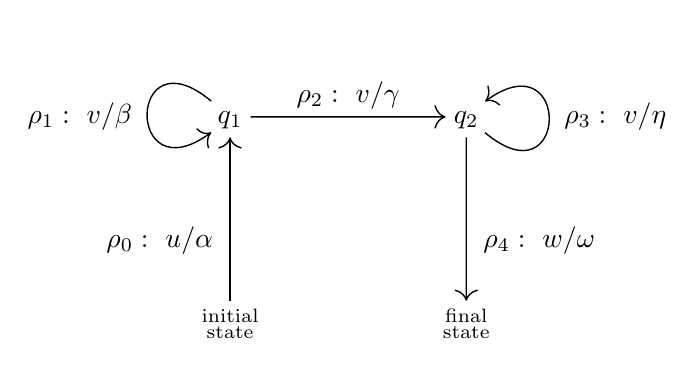
\begin{tikzpicture}[baseline=47, scale=1.5]
	%\draw (-2.75,-0.5) rectangle (4.75,2.5);
	\myclip{-2.75,-0.5}{4.75,2.5}
	%
	\node (q) at (0,1.75) {$q_1$};
	\node (q') at (2,1.75) {$q_2$};
	%
	\node (initial) at (0,0) 
	      {$\begin{subarray}{c} \text{initial} \\ \text{state} \end{subarray}$};
	\node (final) at (2,0) 
	      {$\begin{subarray}{c} \text{final} \\ \text{state} \end{subarray}$};
	%
	\draw (initial) edge [arrow] node [below left=1mm] {$\rho_0: ~u/\alpha~$} (q);
	\draw (q') edge [arrow] node [below right=1mm] {$~\rho_4: ~w/\omega$} (final);
	\draw (q) edge [arrow, loop left] node [left=2mm] {$\rho_1: ~v/\beta$} (q);
	\draw (q) edge [arrow] node [above=1mm] {$\rho_2: ~v/\gamma$} (q');
	\draw (q') edge [arrow, loop right] node [right=2mm] {$\rho_3: ~v/\eta$} (q');
\end{tikzpicture}
\]
where
%, as usual, a notation like $\rho: u'/\mu$ describes 
%a run named $\rho$ that consumes an input $u'$ and produces
%an update $\mu$, and where
the runs $\rho_1$ and $\rho_3$ are loops (in particular,
they produce updates with idempotent skeletons) and
at least two among the runs $\rho_1,\rho_2,\rho_3$ 
are distinct.
\end{definition}

\begin{lemma}\label{lem:finite-ambiguity}
An SST is finite-ambiguous iff 
it does not contain any dumbbell.
\end{lemma}

\begin{proof}
Let 
$T = (\alp, \var, Q, Q_{\mathrm{init}}, Q_{\mathrm{final}}, \finalupd, \Delta)$
be an SST.
\AP
By projecting away the updates on the transitions we obtain from $T$ a 
multiset finite-state automaton $A$.
Formally, $A = (\alp, Q,Q_{\mathrm{init}}, Q_{\mathrm{final}}, \Delta')$,
where $\Delta'$ is the \emph{multiset} containing one occurrence of a
triple $(q,a,q')$ for each transition of the form $(q,a,\alpha,q')$ in $\Delta$.
Note that a multiset automaton can admit several occurrences of 
the same (accepting) run.
Accordingly, the notion of finite ambiguity for $A$ requires the existence
of a uniform bound on the number of \emph{occurrences} of accepting runs
of $A$ on the same input.
We also remark that multiset automata are essentially the same 
as weighted automata over the semiring of natural numbers (the weight of a transition being its number of occurrences), with only a difference in terminology where
finite ambiguity in multiset automata corresponds to 
finite valuedness in weighted automata.

Given the above construction of $A$ from $T$, one can verify by 
induction on $|u|$ that the number of occurrences of accepting runs
of $A$ on $u$ coincides with the number of accepting runs of $T$
on $u$. This means that $A$ is finite-ambiguous iff 
$T$ is finite-ambiguous.

\AP
Finally, we recall the characterizations of finite ambiguity
from \cite{finite-ambiguity1977simon,finite-ambiguity1977jacob,seidl91}
(see in particular Theorem 1.1 and Lemma 2.6 from 
\cite{finite-ambiguity1977simon}).
In short, their results directly imply 
that a multiset automaton is finite-ambiguous iff 
it does not contain a plain dumbbell, namely, a substructure
of the form
\[
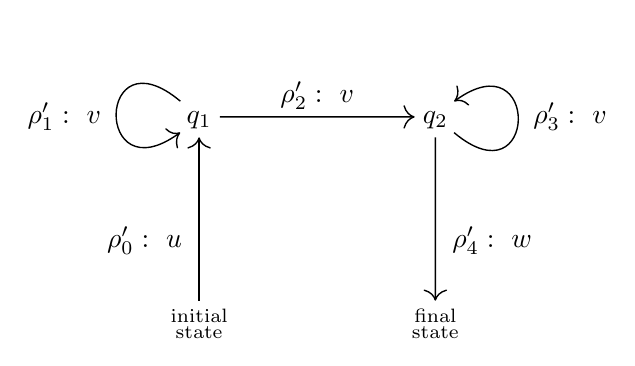
\begin{tikzpicture}[baseline=47, scale=1.5]
	%\draw (-2.5,-0.2) rectangle (4.5,2.25);
	\myclip{-2.5,0}{4.5,2.5}
	%
	\node (q) at (0,1.75) {$q_1$};
	\node (q') at (2,1.75) {$q_2$};
	%
	\node (initial) at (0,0) 
	      {$\begin{subarray}{c} \text{initial} \\ \text{state} \end{subarray}$};
	\node (final) at (2,0) 
	      {$\begin{subarray}{c} \text{final} \\ \text{state} \end{subarray}$};
	%
	\draw (initial) edge [arrow] node [below left=1mm] {$\rho'_0: ~u~$} (q);
	\draw (q') edge [arrow] node [below right=1mm] {$~\rho'_4: ~w$} (final);
	\draw (q) edge [arrow, loop left] node [left=2mm] {$\rho'_1: ~v$} (q);
	\draw (q) edge [arrow] node [above=1mm] {$\rho'_2: ~v$} (q');
	\draw (q') edge [arrow, loop right] node [right=2mm] {$\rho'_3: ~v$} (q');
\end{tikzpicture}
\]
where at least two among $\rho'_1,\rho'_2,\rho'_3$
are distinct  runs.

This almost concludes the proof of the lemma, since any dumbbell 
of $T$ can be projected into a plain dumbbell of $A$.
The converse implication, however, is not completely straightforward.
The reason is that the cyclic runs of a plain dumbbell in $A$
do not necessarily correspond to loops in the SST $T$, 
as the runs need not produce updates 
with idempotent skeletons.
Nonetheless, we can reason as follows.
Suppose that $A$ contains a plain dumbbell, 
with occurrences of runs $\rho'_0,\rho'_1,\rho'_2,\rho'_3,\rho'_4$ 
as depicted above.
Let $\rho_0,\rho_1,\rho_2,\rho_3,\rho_4$ be some
corresponding runs in $T$ (with $\rho_i$ projecting to $\rho'_i$) and let 
$\alpha,\beta,\gamma,\eta,\omega$ be their induced updates.
Further let $n$ be a large enough number such that
$\beta^n$ and $\eta^n$ have idempotent skeletons
(such an $n$ always exists since the skeleton monoid
is finite).
Now consider the substructure in $T$ given by the runs 
$\rho_0$, % $\rho_0= \rho'_0$,
$(\rho_1)^n$, % $\rho_1= (\rho'_1)^n$,
$(\rho_1)^{n-1} \, \rho_2$, %$\rho_2 = %(\rho'_1)^{n-1} \, \rho'_2$,
$(\rho_3)^n$, %$\rho_3 = (\rho'_3)^n$, 
and
$\rho_4$. % $rho_4= \rho'_4$.
This substructure satisfies precisely the definition 
of dumbbell for the SST $T$.
\end{proof}

%
%\christof[inline]{I have made some modifications. However, I am not sure whether it would be better to directly define dumbbells for SSTs and to state the lemma also for SST.}
%\gabriele{Tried to explain, but maybe has to be improved}
%The notion of dumbbell can be readily used on SSTs by allowing arbitrary outputs on the run segments required for a dumbbell. Note that this is different from asking for a dumbbell in the automaton that is obtained from projecting away the outputs: it might me that $\rho_1,\rho_2,\rho_3$ all have the same state/input sequence but differ in the outputs of some transitions. It is not hard to see that Lemma~\ref{lem:finite-ambiguity} also holds for SSTs, so an SST is finite-ambiguous iff it does not contain any dumbbell. 



The second ingredient for the proof of the right-to-left 
implication of Theorem \ref{thm:finite-valued}
uses once more the cover construction 
described in Proposition \ref{prop:separation-covering}.
More precisely, in Lemma \ref{lem:unbounded-values3} below
we show that if an SST $T$ has no simply divergent W-pattern, 
then, for some well chosen values $C$, $D$, $m$, 
the SST $\Cover*[Cm,Dm^2]{T}$ contains no dumbbell.
Before proving the lemma, let us show how it can be used 
to establish the right-to-left implication of Theorem \ref{thm:finite-valued}.

\paragraph{Proof of Theorem~\ref{thm:finite-valued}}
By Lemma~\ref{lem:finite-ambiguity}, 
if $\Cover*[Cm,Dm^2]{T}$ has no dumbbell,
then it is finite-ambiguous, hence %it associates 
%with each input a uniformly bounded %number of outputs.
%In particular, $\Cover*[Cm,Dm^2]{T}$ is
finite-valued.
Since $\Cover*[Cm,Dm^2]{T}$  and $T$ are equivalent,
$T$ is finite-valued, too.
\qed


\begin{lemma}\label{lem:unbounded-values3}
Given an SST $T$, one can compute  numbers $C$, $D$, $m$ such that
if $\Cover*[Cm,Dm^2]{T}$ contains a dumbbell, then $T$ contains a 
simply divergent W-pattern.
\end{lemma}

\begin{proof}
We first provide some intuition. 
If $\Cover[Cm,Dm^2]{T}$ contains a dumbbell for suitable values of $C,D,m$, then we show that
this dumbbell admits two distinct runs $\pi,\pi'$
that have either different outputs or  large delay. 
In both cases we will be able to transform the dumbbell 
into a simply divergent W-pattern in $\Cover[Cm,Dm^2]{T}$, hence $T$ will have one as well.
%For example, in the case of a large %delay, we will rely on 
%Lemmas~\ref{lem:delay-vs-output} and %\ref{lem:ramsey} to 
%identify certain loops in $\pi$ and %$\pi'$ that
%lie entirely inside occurrences of the %runs 
%$\rho_0,\dots,\rho_4$ of the dumbbell, %and 
%such that, when pumped, produce different %outputs. 
%From there, we will be able to expose a %simply divergent 
%W-pattern in $\Cover[Cm,Dm^2]{T}$, and %hence in $T$ as well.


Formally, let $T$ be an SST. Let $C,D$ be defined 
as in Lemma~\ref{lem:delay-vs-output}, and
$m = 7E^{H^2 + H + 1} + 1$, where $E,H$ are 
defined as in Lemma~\ref{lem:ramsey}.
Next, suppose that $\Cover[Cm,Dm^2]{T}$ contains
a dumbbell as in Definition \ref{def:dumbbell}, 
with runs $\rho_0,\rho_1,\rho_2,\rho_3,\rho_4$
that produce respectively the updates
$\alpha,\beta,\gamma,\eta,\omega$. 

Consider the following accepting runs, which are obtained
by composing the copies of the original runs of the dumbbell. The runs $\pi, \pi'$ are different because at least two of $\rho_1,\rho_2,\rho_3$ are different:
\begin{equation}\label{eq:cover-runs}
\begin{aligned}
	\pi  &~=~  \rho_0 ~ \rho_1 ~ \rho_2 ~ \rho_3 ~ \rho_3 ~ \rho_3 ~ \rho_4\\
    \pi' &~=~ \rho_0 ~ \rho_1 ~ \rho_1 ~ \rho_1 ~ \rho_2 ~ \rho_3 ~ \rho_4.
\end{aligned}
\end{equation}
By the properties of $\Cover[Cm,Dm^2]{T}$, 
since $\pi$ and $\pi'$ consume the same input,
they either produce different outputs or
have $Cm$-delay larger than $Dm^2$.

We first consider the case where the outputs are 
different. In this case, we can immediately
witness a simply divergent W-pattern $P$
by adding empty runs to the dumbbell;
formally, for every $i=1,2,3$, we let 
$\rho'_i = \rho_i$ and $\rho''_i = \rho'''_i = \varepsilon$,
so as to form a W-pattern like the one in Figure~\ref{fig:Wpattern}, with
$r_1 = q_1$ and $r_2 = r_3 = q_2$.
Using the notation introduced at the beginning 
of Section \ref{sec:finite-valuedness}, we observe that 
$\pi  = \wrun{1,\underline{1},1,1,1}$ and 
$\pi' = \wrun{1,1,1,\underline{1},1}$
---
recall that the underlined number represents
how many times the small loop at $r_2$,
which is empty here, is repeated along the
run from $q_1$ to $q_2$, and the
other numbers represent how many times the small
loops at $r_1$ and $r_3$, which are also empty here,
are repeated within the occurrences of big loops 
at $q_1$ and $q_2$.
Since, by assumption, the runs $\pi$ and $\pi'$ 
produce different outputs, the W-pattern $P$ 
is simply divergent, as required.

We now consider the case where $\pi$ and $\pi'$
have large delay, namely,
$\delay<C m>{\pi,\pi'} > D m^2$.
In this case Lemma \ref{lem:delay-vs-output} guarantees 
the existence of a set
$I \subseteq \{0, 1, \ldots, |\pi|\}$ containing 
$m$ positions in between the input letters such that,
for all pairs $i < j$ in $I$, the interval $[i,j]$
is a loop on both $\pi$ and $\pi'$ and satisfies
\begin{equation}\label{equ:pumpedDiff}
  \out{\pump<2>[[i,j]]{\pi}} 
  \:\neq\: 
  \out{\pump<2>[[i,j]]{\pi'}}.
\end{equation}

Next, recall from Equation \eqref{eq:cover-runs}
that $\pi$, and similarly $\pi'$, consists of seven parts,
representing copies of the original runs of the dumbbell
and consuming the inputs $u, v, v, v, v, v, w$.
We identify these parts with the numbers $1,\dots,7$.
Since we defined $m$ as $7E^{H^2 + H + 1}+1$,
there is one of these parts
in which at least $E^{H^2 + H + 1}+1$ of the 
aforementioned positions of $I$ occur.
Let $p \in \{1,2,\ldots,7\}$
denote the number of this part,
and let $I_p$ be a set of $E^{H^2 + H + 1}+1$ positions from $I$
that occur entirely inside the $p$-th part.
We conclude the proof by a further case distinction, 
depending on whether $p \in \{1,7\}$ or $p \in \{2,\dots,6\}$.

\paragraph{Parts $1$ and $7$}
Let us suppose that $p \in \{1,7\}$, 
and let $i$ and $j$ be two distinct positions in $I_p$.
We let $P$ be the W-pattern obtained by transforming 
the dumbbell as follows:
\begin{enumerate}
    \item First, we pump either $\rho_0$ or $\rho_4$
          depending on $p$:
    \begin{itemize}
        \item
        If $p = 1$, we set $\rho_0' = \pump<2>[[i,j]]{\rho_0}$
        and $\rho_4' = \rho_4$.
        \item
        If $p = 7$, we set $\rho_4' = \pump<2>[[i-|u\,v^5|,j-|u\,v^5|]]{\rho_4}$
        and $\rho_0' = \rho_0$.
    \end{itemize}
    \item Then, we add empty runs to $\rho_1$, $\rho_2$, and $\rho_3$;
    formally, for each $h \in \{1,2,3\}$, we set
    $\rho_h' = \rho_h$ and $\rho_h'' = \rho_h''' = \varepsilon$.
\end{enumerate}
Now that we identified a W-pattern $P$ in $\Cover{T}$, 
we note that 
\[
\begin{aligned}
  \pump<2>[[i,j]]{\pi}  &~=~ \wrun{1,\underline{1},1,1,1} \\
  \pump<2>[[i,j]]{\pi'} &~=~ \wrun{1,1,1,\underline{1},1}.
\end{aligned}
\]
We also recall Equation~\ref{equ:pumpedDiff}, which states 
that these runs produce different outputs.
This means that the W-pattern $P$ is simply divergent.
Finally, since the runs of $\Cover{T}$ can be projected 
into runs of $T$, we conclude that $T$ contains a 
simply divergent W-pattern.


\paragraph{Parts $2 - 6$}
Let us suppose that $p \in \{2,\dots,6\}$.
Note that, in this case, the elements of $I_p$ 
denote positions inside the $p$-th factor of the input
$u\,v\,v\,v\,v\,v\,w$, which is a $v$.
To refer directly to the positions of $v$, we define
$I'_p$ as the set obtained by subtracting $|u\,v^{p-1}|$ 
from each element of $I_p$.
Since the set $|I'_p|$ has cardinality $E^{H^2 + H + 1}+1$,
we claim that we can find an interval with endpoints from $I'_p$ 
that is a loop of $\rho_1$, $\rho_2$, and $\rho_3$, at the same time.
Specifically, we can do so via three consecutive applications 
of Lemma~\ref{lem:ramsey}:
\begin{enumerate}
    \item As $|I'_p| = E^{H^2 + H + 1}+1 = E \cdot (E^{H+1})^H + 1$,
    there exists a set $I''_p \subseteq I'_p$ of cardinality $E^{H+1}+1$
    such that for every pair $i < j$ in $I''_p$, the interval $[i,j]$
    is a loop of $\rho_1$;
    \item As $|I_p''| = E^{H+1}+1 = E \cdot E^H + 1$,
    there exists $I'''_p \subseteq I''_p$ of cardinality $E+1$
    s.t. for every pair $i < j$ in $I'''_p$, the interval $[i,j]$
    is a loop of $\rho_2$ 
    (and also of $\rho_1$, since $i,j \in I'''_p \subseteq I''_p$);
    \item As $|I'''_p| = E + 1 = E \cdot 1^H + 1$, 
    there are two positions $i<j$ in $I'''_p$
    such that the interval $[i,j]$ is a loop of $\rho_3$ 
    (and also of $\rho_1$ and $\rho_2$ since $i,j \in I'''_p \subseteq I''_p$).
\end{enumerate}
The diagram below summarizes the current situation:
we have just managed to find an interval $[i,j]$ 
that is a loop on all $v$-labelled runs 
$\rho_1,\rho_2,\rho_3$ 
of the dumbbell (the occurrences of this interval
inside $\rho_1,\rho_2,\rho_3$ are highlighted by thick
segments):
\[
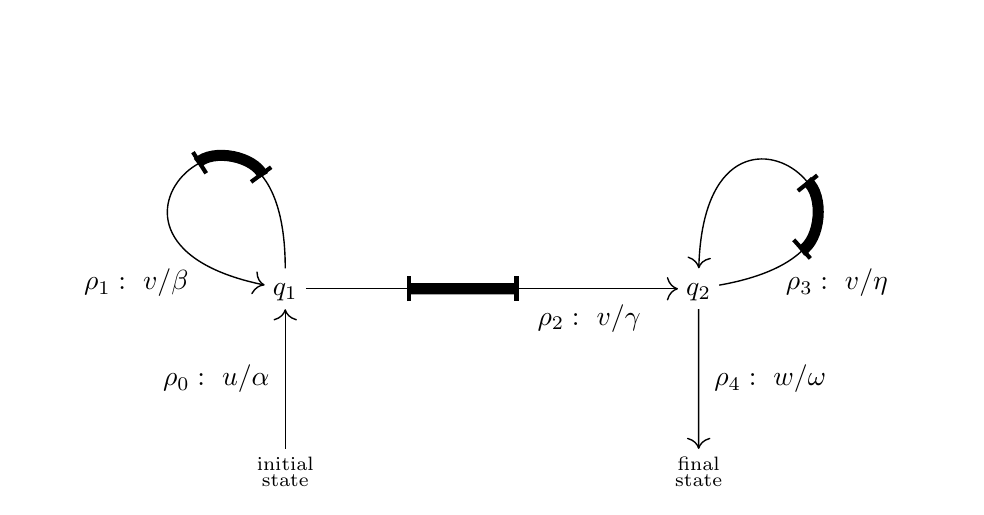
\begin{tikzpicture}[scale=1.5]
%\draw (-2.6,-0.3) rectangle (6.1,3.5);
\myclip{-2.6,-0.3}{6.1,3.5}
%
\node (initial) at (0,0.1) 
	  {$\begin{subarray}{c} \text{initial} \\ \text{state} \end{subarray}$};
\node (q) at (0,1.65) {$q_1$};
\node (q') at (3.5,1.65) {$q_2$}; 
\node (final) at (3.5,0.1) 
	  {$\begin{subarray}{c} \text{final} \\ \text{state} \end{subarray}$};
%
\draw (initial) edge [arrow] 
      node [left=2mm] {$\rho_0:~ u/\alpha$} (q);
\draw (q') edge [arrow] 
      node [right=2mm] {$\rho_4:~ w/\omega$} (final);
\draw (q) edge [arrow,  looseness=40, out=90, in=170]      
	  node [below left, pos=.9] {$\rho_1:~ v/\beta\phantom{xi}$} 
      node [pos=.15] (i) {}
      node [pos=.5] (j) {}
      (q);
\draw (q') edge [arrow,  looseness=40, out=10, in=90]             
	  node [below right, pos=.1] {$\phantom{x}\rho_3:~ v/\eta$} 
      node [pos=.15] (i'') {}
      node [pos=.5] (j'') {}
      (q');
\draw (q) edge [arrow]             
	  node [below = 2mm, pos=.75] {$\rho_2:~ v/\gamma$} 
      node [pos=.25] (i') {}
      node [pos=.6] (j') {}
      (q');
%
\draw (i) edge [bend right = 55, line width=4] (j);
\draw (i) edge [|-|, bend right = 55, line width=1.5] (j);
\draw (i') edge [line width=4] (j');
\draw (i') edge [|-|, line width=1.5] (j');
\draw (i'') edge [bend right = 55, line width=4] (j'');
\draw (i'') edge [|-|, bend right = 55, line width=1.5] (j'');
\end{tikzpicture}
\]


We can now expose a W-pattern $P$ by merging the
positions $i$ and $j$ inside each $v$-labelled run 
$\rho_1$, $\rho_2$, and $\rho_3$ of the dumbbell.
Formally, we let 
$\rho'_0 = \rho_0$, 
$\rho'_4 = \rho_4$, and for every $h \in \{1,2,3\}$,
we define $\rho'_h$, $\rho''_h$, and $\rho'''_h$, respectively,
as the intervals $[0,i]$, $[i,j]$, and $[j,|v|]$ of $\rho_h$.
%Note that this W-pattern is well defined since the three $\rho_h[i,j]$ are loops. 
Now that we have identified a W-pattern $P$ inside $\Cover{T}$,
we remark that 
$\pi  = \wrun{1,\underline{1},1,1,1}$ and 
$\pi' = \wrun{1,1,1,\underline{1},1}$.
Additionally, if we transpose $i$ and $j$ from $I_p'$ back to $I$,
that is, if we set $i' = i+|u\,v^{p-1}|$ and $j' = j+|u\,v^{p-1}|$,
since both $i'$ and $j'$ occur in the $p$-th part of $\pi$ and $\pi'$,
pumping the interval $[i',j']$ in $\pi$ (resp.~$\pi'$) amounts to 
incrementing the $(p-1)$-th parameter in the notation
$\wrun{1,\underline{1},1,1,1}$ (resp.~$\wrun{1,1,1,\underline{1},1}$).
More precisely:
\[
\begin{aligned}
  \pump<2>[[i',j']]{\pi}   &~=~ \wrun{n_1,\underline{n_2},n_3,n_4,n_5} \\
  \pump<2>[[i',j']]{\pi'}  &~=~ \wrun{n_1,n_2,n_3,\underline{n_4},n_5}
\end{aligned}
\]
where each $n_{p'}$ is either $2$ or $1$ depending on whether $p' = p-1$ or not.
Since Equation~\ref{equ:pumpedDiff} states that these two runs 
produce different outputs, the W-pattern $P$ is simply divergent.
Finally, since the runs of $\Cover{T}$ can be projected 
into runs of $T$, we conclude that, also in this case, 
$T$ contains a simply divergent W-pattern.
\end{proof}





\section{Conclusion}\label{sec:conclusion}

We have drawn a rather complete
picture of finite-valued SSTs and answered several open questions of~\cite{DBLP:conf/icalp/AlurD11}. 
Regarding expressiveness, finite-valued SSTs can be decomposed as unions of deterministic SSTs
(Theorem~\ref{thm:FiniteValuedToDecomposition}). They are
equivalent to finite-valued two-way transducers
(Theorem~\ref{thm:finval-SST-2FT}), and to finite-valued
non-deterministic MSO
transductions (see Section~\ref{sec:intro}). On the algorithmic side,
their equivalence problem is decidable in elementary time
(Theorem~\ref{thm:equiv-finval-SST}) and finite valuedness of SSTs is
decidable in {\upshape\sc PSpace} ({\upshape\sc PTime} for fixed number of
variables), see Theorem~\ref{thm:effectiveness}. As an alternative proof
to the result of~\cite{YenY22}, our results imply that finite valuedness of
two-way transducers can be decided in
{\upshape\sc PSpace} 
(Corollary~\ref{thm:finval-twoway}). Because of the effective expressiveness
equivalence between SSTs and non-deterministic MSO transductions, our
result also entails decidability of finite valuedness for the latter
class.


\medskip
\subparagraph{\bf Further questions.}
A first natural question is how big the valuedness of an SST can
be.
In the classical case of one-way transducers the valuedness has been
shown to be at most exponential (if finite)~\cite{Weber93}.
We can obtain a bound from Lemma~\ref{lem:unbounded-values3}, but the
value is likely to be sub-optimal.


Our equivalence procedure relies on the
decomposition of a $k$-valued SST into a union of $k$ deterministic
SSTs each of elementary size. The latter construction is likely to
be sub-optimal, too, and so is our complexity for checking equivalence. 
%On the other hand, only a {\upshape\sc PSpace} lower bound is
%known~\cite{equivalence-finite-valued}. 
On the other hand, only a {\upshape\sc PSpace} lower bound is
known, which follows easily from a reduction of NFA equivalence~\cite{AhoHU74}. 
A better understanding of the
complexity of the equivalence problem for (sub)classes of SSTs is a
challenging question. Already for deterministic SSTs, the complexity of the equivalence problem
is only known to lie between {\upshape\sc NLogSpace} and
{\upshape\sc PSpace}~\cite{DBLP:conf/popl/AlurC11}.

However, beyond the finite-valued setting there is little hope to 
find a natural restriction on valuedness which would preserve 
the decidability of the equivalence problem. Already for 
one-way transducers of linear valuedness (i.e.~where the number 
of outputs is linear in the input length), equivalence is
undecidable, as shown through a small modification of the 
proof of~\cite{iba78siam}. 


Deterministic SSTs have been extended,
while preserving decidability of the equivalence problem,
in several ways:
to copyful SSTs~\cite{DBLP:journals/siglog/Bojanczyk19a,DBLP:journals/fuin/FiliotR21},
which allow to copy the content of variables several times, 
to infinite strings~\cite{DBLP:conf/lics/AlurFT12}, and to
trees~\cite{DBLP:journals/jacm/AlurD17}. 
Generalizations of these results to the finite-valued setting 
yield interesting questions. On trees, similar questions 
(effective finite valuedness, decomposition and equivalence) 
have been answered positively for bottom-up tree
transducers~\cite{DBLP:journals/mst/Seidl94}.


Finally, SSTs have linear input-to-output growth (in the length of the
strings). There is a recent trend in extending transducer models 
to allow polynomial growth
\cite{DBLP:conf/icalp/BojanczykKL19,DBLP:conf/lics/Bojanczyk22,DBLP:conf/lics/Bojanczyk23a,GaetanPhD}.
Finite valuedness has not  been studied in this context yet.


    \bibliographystyle{plainnat}\bibliography{biblio}

% \bibliographystyle{plainurl}
% \bibliography{biblio}

\end{document}

%%% Local Variables:
%%% mode: latex
%%% TeX-master: t
%%% End:
